\documentclass{beamer}

% \usepackage{xcolor}
% \definecolor{darkred}{rgb}{0,0,1}

\mode<presentation>
{
  \usetheme{CambridgeUS}
  \usecolortheme{beaver}
  \usefonttheme{default}
  \setbeamertemplate{navigation symbols}{}
  \setbeamertemplate{caption}[numbered]
  \setbeamertemplate{itemize item}{\color{darkred}$\blacktriangleright$}
  \setbeamertemplate{itemize subitem}[square]
  \setbeamertemplate{itemize subsubitem}[square]
  \setbeamertemplate{enumerate item}[square]
  \setbeamertemplate{sections/subsections in toc}[square]
  \setbeamercolor{section number projected}{bg=darkred,fg=white}
} 

\usepackage[english]{babel}
\usepackage[utf8]{inputenc}
\usepackage[T1]{fontenc}
\usepackage{enumerate}
\usepackage{amsmath}
\usepackage{graphicx}
\graphicspath{{figures/}{symsimquality/}{adobe/}{modelcheck/}}

\usepackage[sort, numbers]{natbib}
\bibliographystyle{unsrt}

\usepackage{tikz}
\usetikzlibrary{bayesnet}
\usepackage{amsthm}
\usepackage{amssymb}
\usepackage{amsfonts}
\tikzset{>=latex}
\usepackage{bm}

\def\mywarn#1{\textcolor{red}{#1}}
\def\myemph#1{\textcolor{blue}{#1}}
\def\mycell#1{\textcolor{brown}{#1}}

\AtBeginSubsection[] {
  \begin{frame}<beamer>{Outline}
    \tableofcontents[currentsection,currentsubsection]
  \end{frame}
}

\title[mssc]{\myemph{M}ultiple-\myemph{S}ample Differential
  Expression Analysis for \myemph{S}ingle-\myemph{C}ell RNA Sequencing Data}
\author{Songpeng Zu}
\date{\today}

\begin{document}

\begin{frame}
  \titlepage
\end{frame}

\begin{frame}{Outline}
  \tableofcontents[hideallsubsections]
  % \tableofcontents
\end{frame}

\section{Introduction}
\subsection*{Multi-sample scRNASeq DE analysis}

\begin{frame}
  Finding genes that are differentially expressed (\mywarn{shift of the mean}) under
  different conditions. 
  \begin{columns}
    \begin{column}{0.6\textwidth}
      \begin{figure}
        \centering
        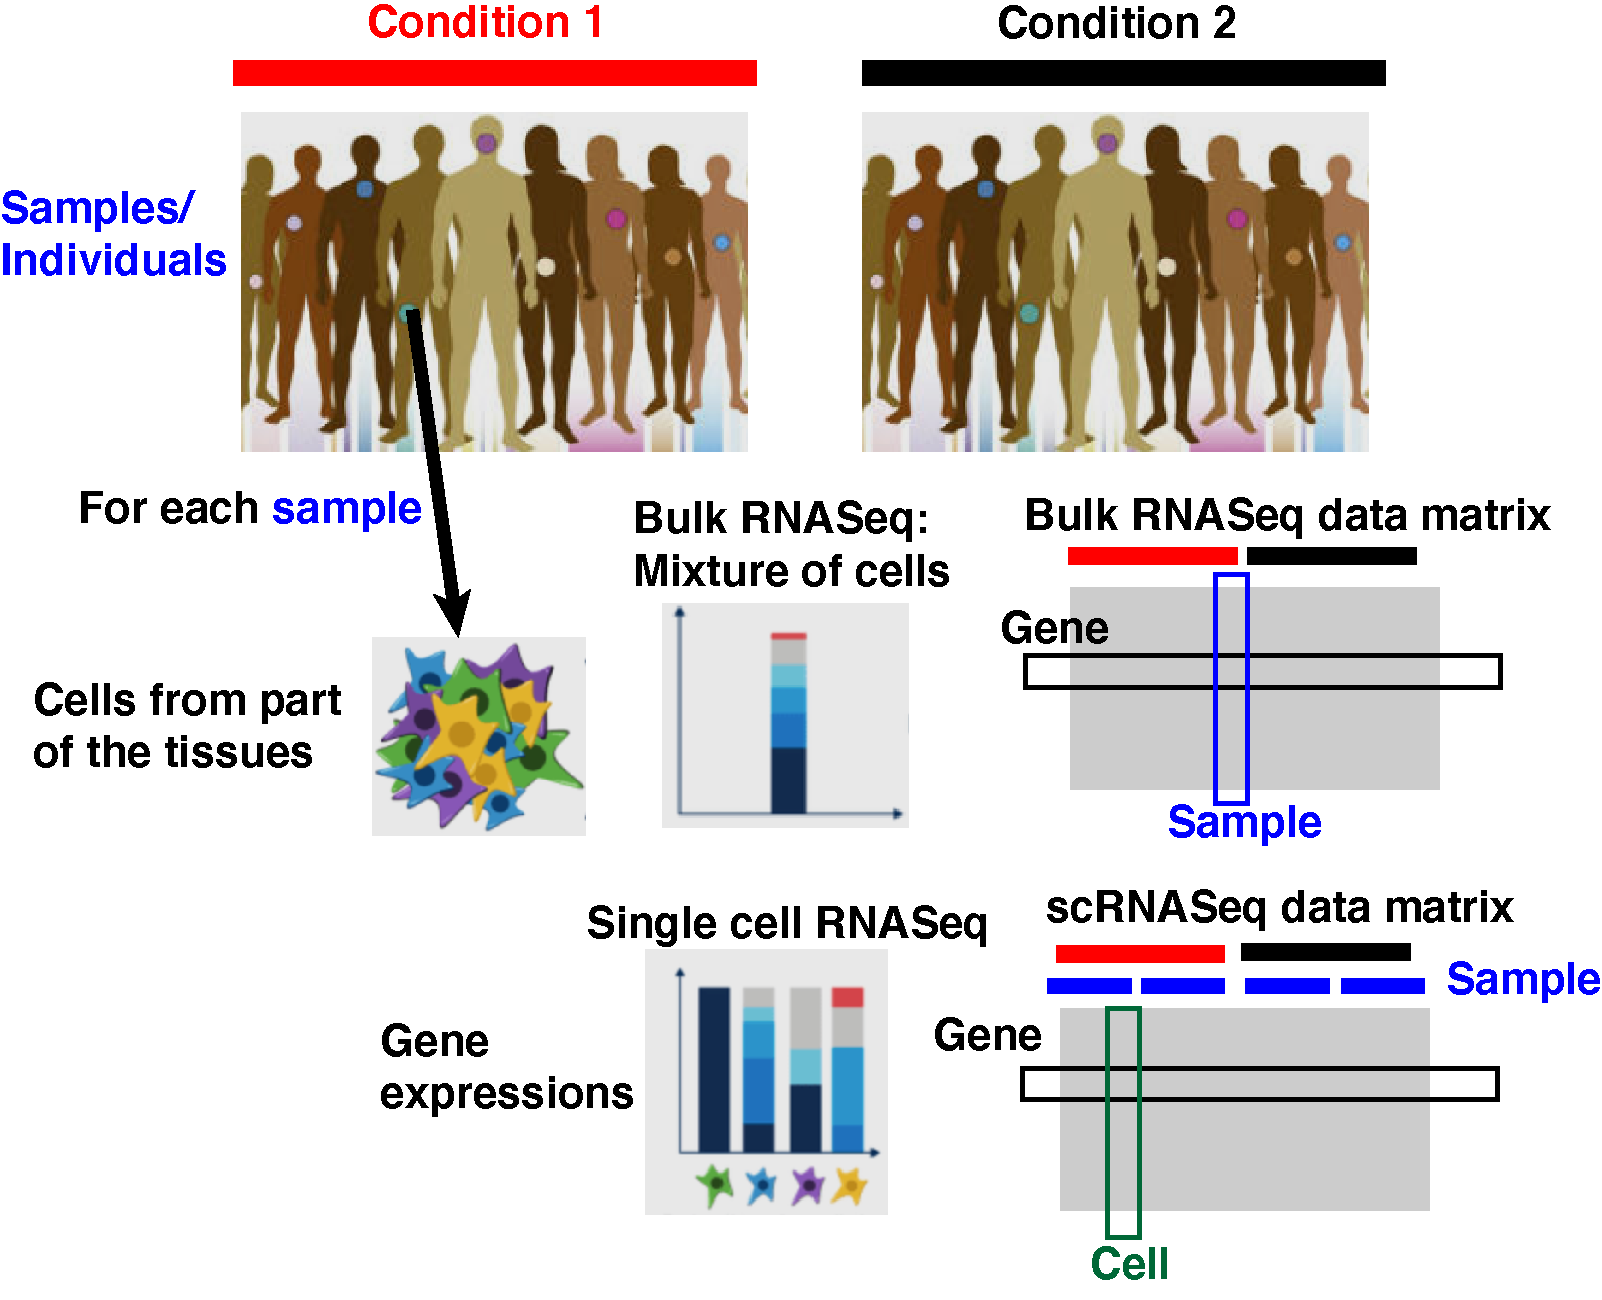
\includegraphics[width = \textwidth]{background_explain}
      \end{figure}
    \end{column}
    \begin{column}{0.45\textwidth}
      \begin{itemize}
      \item Bulk RNASeq: \\the gene \(i\) in the sample \(j\)
        \({\scriptstyle \log_2CPM(X_{ij}) = \log_2(1 + X_{ij} \cdot S_{j}) }\) \\
        \({\scriptstyle S_j =\frac{1}{\sum_{i} X_{ij}} \cdot 10^6}\)
    \item UMI-based scRNAseq
      \begin{itemize}
      \item Data: 70\% zeros
      \item Limited samples
      \item Technical variations:\\
        1. Batch effect\\
        2. scRNA sequencing
      \item Biological variations:\\
        1. Genetic background \\
        2. Cell heterogeneity
         \end{itemize}
      \end{itemize}
    \end{column}
  \end{columns}
\end{frame}

\begin{frame}
  \begin{figure}
    \centering
    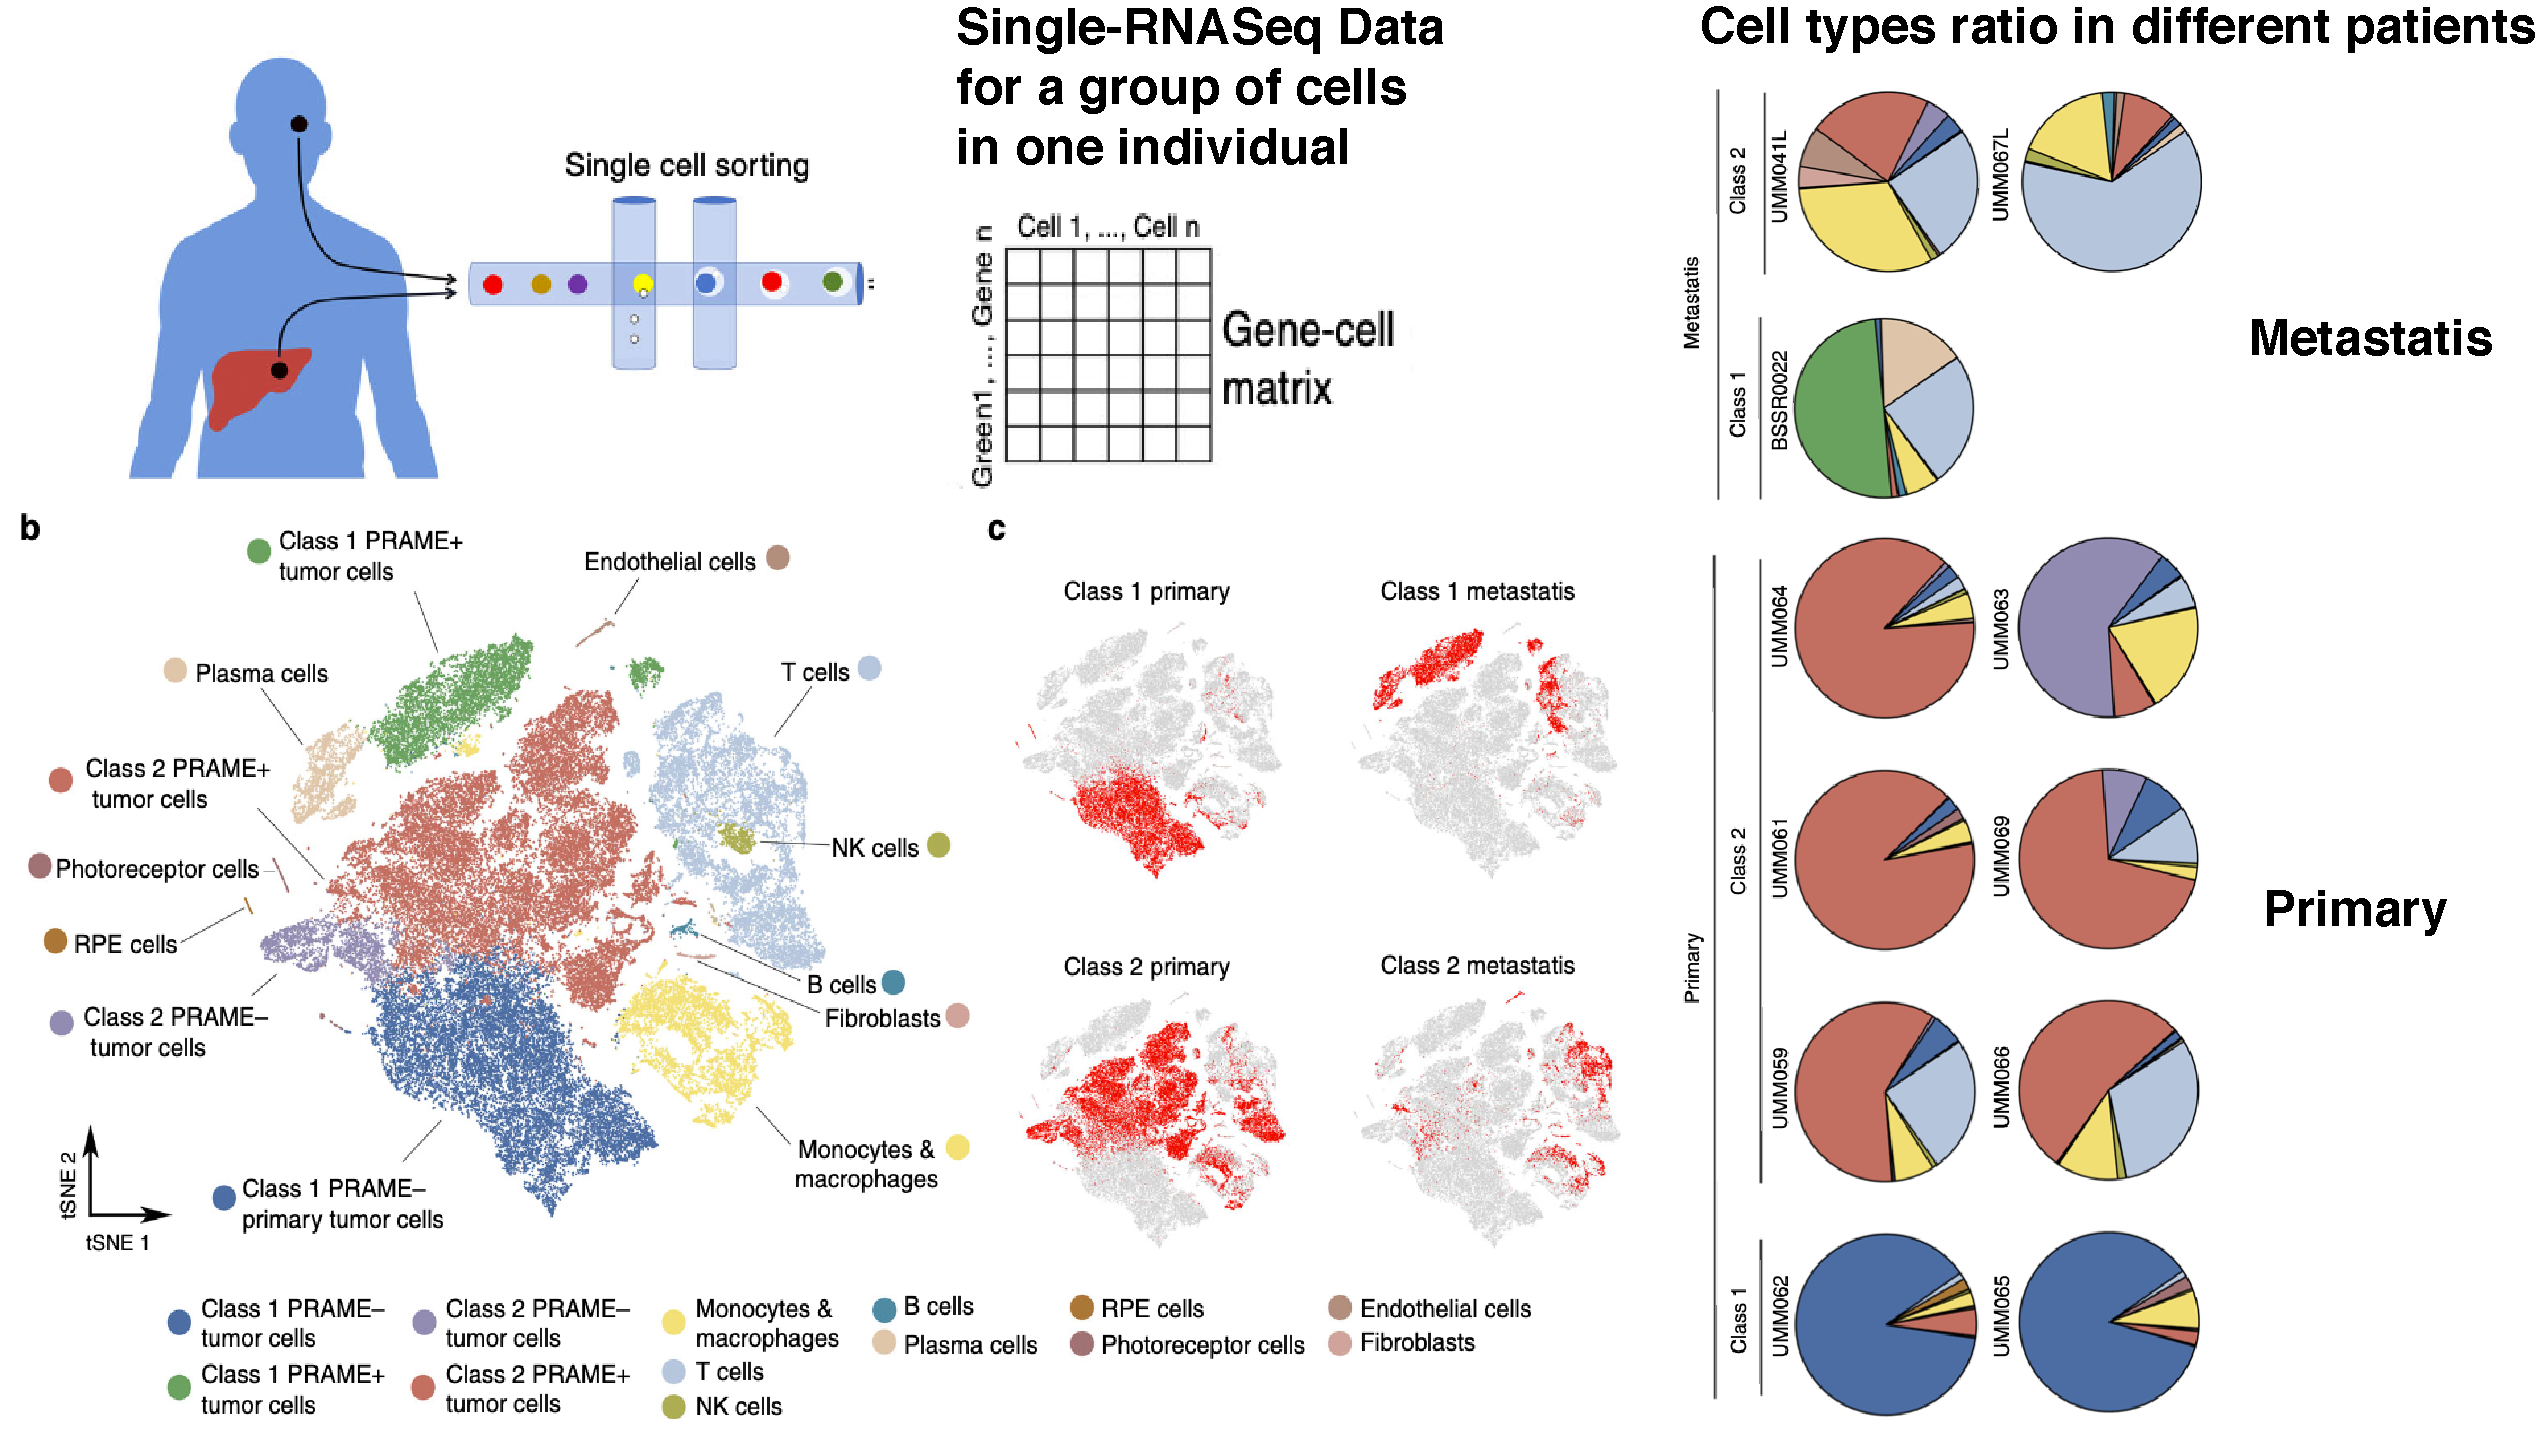
\includegraphics[width = \textwidth]{intro_overview}
    \caption{Multiple-sample scRNAseq Data \cite{durante2020single}.}
  \end{figure}
\end{frame}

\begin{frame}
  \begin{figure}
    \centering
    \includegraphics[width = 0.9\textwidth]{patient-specific.png}
    \caption{DE analysis on one cell sub-population inferred by Harmony
      \cite{korsunsky2019fast}}
  \end{figure}
\end{frame}

\begin{frame}
  \begin{figure}
    \centering
    \includegraphics[width=\textwidth]{pseudobulkwhenmorezeros}
    \caption{Pseudo-bulk analysis \cite{schmid2020design} on PBMC dataset.}
  \end{figure}
\end{frame}



\section{Model}
\subsection{A general framework}
\begin{frame}{Modeling the mean}
  Let \(X_{ij}\) represent the UMI counts for the gene \(i\) in the cell \(j\)
  \begin{align}
    X_{ij} \sim f(\mu_{ij}, \phi_i) \\
    \mu_{ij}  = S_j * \lambda_{ij} \\
    g^{-1}(\lambda_{ij})  = \sum_r d_{jr} \beta_{ir} \\
    \bm{\beta_i} \sim {\cal N}(\bm{0}, \bm{\Lambda})
  \end{align}
  A typical content in $\mathbf{d_j}$ is followed:
  \begin{equation*}
   \mathbf{d_j} = \left(1, \overbrace{(0, 1, \dots, 0, 0)}^{\text{\myemph{individual} one-hot vector}}, \underbrace{(1, 0)}_{\text{\mywarn{conditional} one-hot vector}}\right)
  \end{equation*}
\end{frame}

\subsection{UMI Count vs TPM}

\begin{frame}
  \frametitle{UMI-Count vs TPM}
  \begin{itemize}
  \item
    Data set: PBMC scRNAseq data \cite{yuen2020high}, 10 individuals, 5 vs 5 in
    two conditions.
  \item
    Select genes:
    \begin{itemize}
    \item
      DEGs: CCL4L1, CCL4L2, CCL3L1, CCL3L3
    \item
      Genes with lots of zeros: MIR155HG, TNFRSF4, ICAM1, NA.499, HIST2H2AA4
    \item
      Genes with strong individual effects: HBB, HBA2, HBA1 
    \end{itemize}
  % \item
    % \(\log_2CPM\) for the gene \(i\) in the cell is defined as \(log_2(\frac{X_g}{\sum_g X_g} \times C + 1)\), C is a
    % constant, defined as \(10^4\) in Seurat.
  \end{itemize}
\end{frame}

\begin{frame}
  \frametitle{What is a violin plot?}
  Violin plots are similar to box plots, except that they also show the kernel
  probability density of the data at different values.
  \begin{figure}
    \centering
    \includegraphics[width = 0.8\textwidth]{violin_figure_case}
    \caption{Violin plot. Left: Dotplot, where each dot corresponds to one
      sample; Right: Jitter plot, which adds small randomness to the data in
      order to reduce the overlap among the points.}
  \end{figure}
\end{frame}

\begin{frame}
  \frametitle{DEGs in all cells}
  \begin{figure}
    \centering
    \includegraphics[width=\textwidth]{vln_cnt-tpm_DEGs_allcells}
  \end{figure}
\end{frame}

\begin{frame}
  \frametitle{DEGs in cytotoxic T cells}
  \begin{figure}
    \centering
    \includegraphics[width=\textwidth]{vln_cnt-tpm_DEGs_cytotoxicTcell}
  \end{figure}
\end{frame}

\begin{frame}
\frametitle{Genes with lots of zeros in all cells}
\begin{figure}
  \centering
  \includegraphics[width=\textwidth]{vln_cnt-tpm_heavyzeros_allcells}
\end{figure}
\end{frame}

\begin{frame}
  \frametitle{Genes with lots of zeros in cytotoxic T cells}
  \begin{figure}
    \centering
    \includegraphics[width=\textwidth]{vln_cnt-tpm_heavyzeros_cytotoxicTcell}
  \end{figure}
\end{frame}

\begin{frame}
\frametitle{Genes with strong individual effects in all cells}
\begin{figure}
  \centering
  \includegraphics[width=\textwidth]{vln_cnt-tpm_heavyindeff_allcells}
\end{figure}
\end{frame}

\begin{frame}
  \frametitle{Genes with strong individual effects in cytotoxic T cells}
  \begin{figure}
    \centering
    \includegraphics[width=\textwidth]{vln_cnt-tpm_heavyindeff_cytotoxicTcell}
  \end{figure}
\end{frame}

\begin{frame}
  \frametitle{Multinomial model on scRNASeq \cite{townes2019feature}}
  Under a multinomial distribution on the observed UMI counts, 74\%-90\%
  zeros, 22-30\% ones, and less than 4\% values above one. This will
  artificially enhance the gap between zero and nonzeros values on
  log-normalized data.
  \begin{figure}
    \centering
    \includegraphics[width=\textwidth]{lognorm_artificial_zeroinflation}
  \end{figure}
\end{frame}


\subsection{Modeling UMI count}
\begin{frame}
  For any given gene, the UMI count \(X_j\) in the cell \(j\),   \(S_j\) is the
  scale factor for the cell \(j\), which reflect the sequencing depth in the
  cell \(j\). 
  \begin{align}
    X_{j} &\sim {\it Poisson}(\lambda) \\
    X_{j} &\sim {\it Poisson}(\myemph{S_j}\cdot\tilde{\lambda}) \\
    X_{j} &\sim {\it PoissonlogNormal}(\mu, \sigma^2) \nonumber \\
         &= \int_{\lambda} Poisson(X|\myemph{S_j}\cdot \lambda)\cdot logNormal(\lambda | \mu,\sigma^2) \\
    X_{j} &\sim {\it Negative Binomial} (\myemph{S_j}\cdot\mu, \phi)
  \end{align}
  \begin{itemize}
\item
  In NB distribution, we use the mean \(\mu\) and
  dispersion \(\phi\) (namely \(r\)) , and then the variance \(\sigma^2 = \mu +
  \mu^2/\phi\), and the success probability \(p = \frac{\mu}{\mu + \phi}\).
\item
  NB can be treated as Gamma-Poisson mixture, i.e., \({\scriptstyle NB(\mu,\phi)=\int_\lambda
  Poisson(\lambda)Gamma(\phi, \phi/\mu)}\), in which, \(\phi\) is the shape, and
  \(\phi/\mu\) is the rate parameter in Gamma distribution.
\end{itemize}
\end{frame}

\begin{frame}{One cell subpopulation from one individual}
  \begin{table}
    \centering
    \begin{tabular}{c|c|c|c|c|c|c}
      Gene & Obs & Poi & Pois & Poilognm & Poislognm & NB \\
      \hline
      CCL4L1    & 0.840& 0.813& 0.824& 0.843& 0.850& 0.842 \\
      CCL4L2    & 0.837& 0.810& 0.822& 0.840& 0.847& 0.839 \\
      CCL3L1    & 0.729& \mywarn{0.403}& \mywarn{0.429}& 0.727& 0.734& 0.737 \\
      CCL3L3    & 0.729& \mywarn{0.404}& \mywarn{0.430}& 0.727& 0.734& 0.736 \\
      MIR155HG  & 0.961& 0.953& 0.956& 0.960& 0.962& 0.961 \\
      TNFRSF4   & 0.958& 0.959& 0.962& 0.959& 0.962& 0.959 \\
      ICAM1     & 0.952& 0.938& 0.942& 0.951& 0.953& 0.952 \\
      NA.499    & 0.971& 0.971& 0.973& 0.971& 0.973& 0.971 \\
      HIST2H2AA4& 0.942& 0.944& 0.948& 0.944& 0.948& 0.944 \\
      HBB       & 0.661& \mywarn{0.445}& \mywarn{0.470}& 0.621& 0.624& \myemph{0.644} \\
      HBA2      & 0.785& \mywarn{0.670}& \mywarn{0.689}& 0.765& 0.768& 0.779 \\
      HBA1      & 0.875& 0.863& 0.871& 0.872& 0.878& 0.874 \\
      \hline
    \end{tabular}
    \caption{Zero ratio estimations for cells from Cluster 2, the individual R1}
  \end{table}
\end{frame}

\begin{frame}{Two cell subpopulations from one individuals}
  \begin{table}
    \centering
    \begin{tabular}{c|c|c|c|c|c|c}
      Gene & Obs & Poi & Pois & Poilognm & Poislognm & NB \\
      \hline
      CCL4L1    & 0.961& 0.953& 0.957& 0.960& 0.963& 0.961\\ 
      CCL4L2    & 0.960& 0.952& 0.956& 0.959& 0.962& 0.960\\
      CCL3L1    & 0.802& \mywarn{0.689}& \mywarn{0.711}& 0.798& 0.806& 0.803\\
      CCL3L3    & 0.802& \mywarn{0.689}& \mywarn{0.711}& 0.798& 0.806& 0.803\\
      MIR155HG  & 0.990& 0.989& 0.990& 0.990& 0.990& 0.990\\
      TNFRSF4   & 0.989& 0.989& 0.990& 0.989& 0.990& 0.989\\
      ICAM1     & 0.803& 0.783& 0.800& 0.802& 0.812& 0.803\\
      NA.499    & 0.920& 0.921& 0.928& 0.921& 0.928& 0.921\\
      HIST2H2AA4& 0.901& 0.900& 0.908& 0.901& 0.908& 0.901\\
      HBB       & 0.486& \mywarn{0.204}& \mywarn{0.234}& \mywarn{0.423}& \mywarn{0.412}& \myemph{0.457}\\
      HBA2      & 0.535& \mywarn{0.333}& \mywarn{0.365}& \mywarn{0.496}& \mywarn{0.492}& \myemph{0.520}\\
      HBA1      & 0.716& 0.653& 0.677& 0.705& 0.711& 0.712\\
      \hline 
    \end{tabular}
    \caption{Zero ratio estimations for cells from Cluster 1 and 2, the
      individual R1}
  \end{table}
\end{frame}

\begin{frame}{One cell subpopulation from all the individuals}
  \begin{table}
    \centering
    \begin{tabular}{c|c|c|c|c|c|c}
      Gene & Obs & Poi & Pois & Poilognm & Poislognm & NB \\
      \hline
      CCL4L1    & 0.953& 0.946& 0.958& 0.953& 0.962& 0.953\\ 
      CCL4L2    & 0.952& 0.945& 0.957& 0.952& 0.961& 0.953\\
      CCL3L1    & 0.925& \mywarn{0.871}& \mywarn{0.899}& 0.924& 0.934& 0.925\\
      CCL3L3    & 0.925& \mywarn{0.871}& \mywarn{0.899}& 0.924& 0.934& 0.925\\
      MIR155HG  & 0.985& 0.984& 0.987& 0.985& 0.988& 0.985\\
      TNFRSF4   & 0.978& 0.977& 0.982& 0.978& 0.982& 0.978\\
      ICAM1     & 0.965& 0.962& 0.971& 0.965& 0.972& 0.965\\
      NA.499    & 0.987& 0.987& 0.990& 0.987& 0.990& 0.987\\
      HIST2H2AA4& 0.948& 0.945& 0.957& 0.948& 0.958& 0.948\\
      HBB       & 0.911& \mywarn{0.469}& \mywarn{0.557}& \mywarn{0.892}& 0.907& \myemph{0.911}\\ 
      HBA2      & 0.934& \mywarn{0.763}& \mywarn{0.811}& 0.921& 0.932& 0.933\\
      HBA1      & 0.941& \mywarn{0.867}& \mywarn{0.895}& 0.936& 0.945& 0.941\\
     \hline 
    \end{tabular}
    \caption{Zero ratio estimations for cells from Cluster2, 10 individuals.}
  \end{table}
  
\end{frame}


\begin{frame}{Two cell subpopulations from all the individuals}
  \begin{table}
    \centering
    \begin{tabular}{c|c|c|c|c|c|c}
      Gene & Obs & Poi & Pois & Poilognm & Poislognm & NB \\
      \hline
      CCL4L1    & 0.969& 0.965& 0.974& 0.969& 0.975& 0.969\\ 
      CCL4L2    & 0.969& 0.964& 0.974& 0.969& 0.975& 0.969\\
      CCL3L1    & 0.857& \mywarn{0.761}& 0.819& 0.856& 0.873& 0.858\\
      CCL3L3    & 0.857& \mywarn{0.761}& 0.819& 0.856& 0.873& 0.858\\
      MIR155HG  & 0.991& 0.990& 0.993& 0.990& 0.992& \mywarn{NA}   \\
      TNFRSF4   & 0.986& 0.985& 0.989& 0.986& 0.989& 0.986\\
      ICAM1     & 0.873& 0.857& 0.893& 0.871& 0.897& 0.872\\
      NA.499    & 0.926& 0.916& 0.938& 0.926& 0.941& 0.926\\
      HIST2H2AA4& 0.901& 0.887& 0.916& 0.901& 0.921& 0.901\\
      HBB       & 0.823& \mywarn{0.289}& \mywarn{0.403}& 0.812& 0.819& 0.823\\
      HBA2      & 0.846& \mywarn{0.583}& \mywarn{0.674}& 0.838& 0.844& 0.844\\
      HBA1      & 0.890& 0.775& 0.830& 0.887& 0.898& 0.890\\
    \end{tabular}
    \caption{Zero ratio estimation for cells from Cluster 1 and 2, 10
      individuals.}
  \end{table}
\end{frame}


\begin{frame}
  \begin{figure}
    \centering
    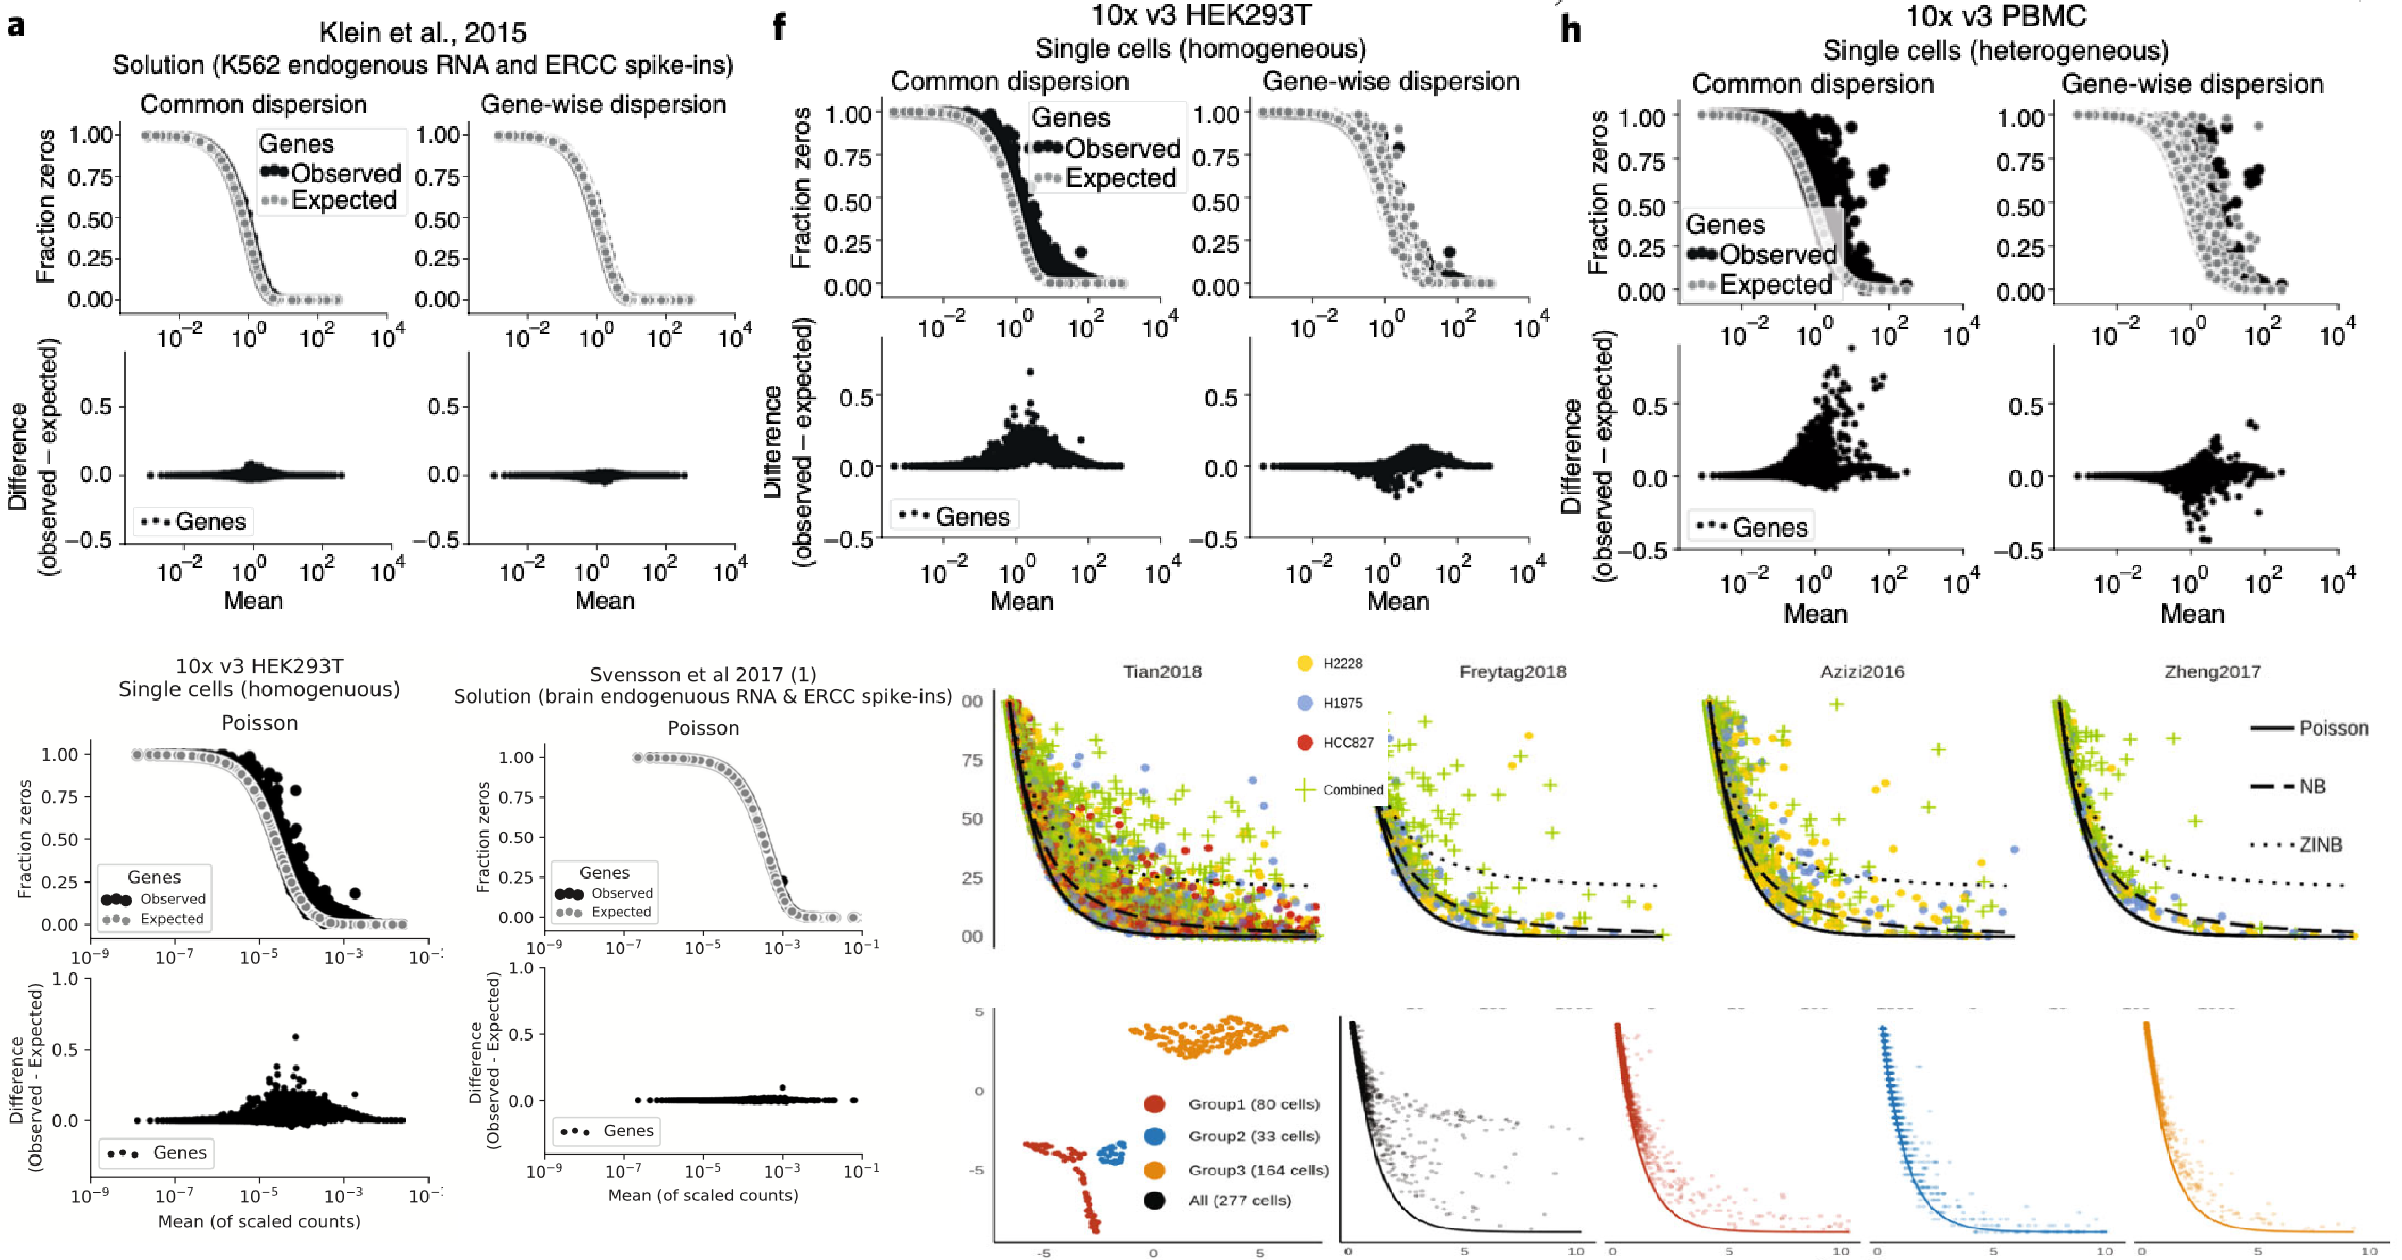
\includegraphics[width = \textwidth]{not_tech_zero_inflation}
    \caption{Observed and expected zeros with NB, Poisson or Poisson with scaled
    mean. Grey figures from \cite{svensson2020droplet}; color
    figures from \cite{kim2020demystifying}.}
  \end{figure}
\end{frame}

\begin{frame}
  \frametitle{Modeling scRNAseq Using Negative Binomial}
  \begin{itemize}
  \item
    We need the dispersion \(\phi\) for each gene to model the variance of gene
    expression 
    due to heterogeneity. In reality, we cannot get a group of homogeneous
    cells\footnote{Cell annotation itself is now a really hot topic in scRNAseq
      data analysis.}. Meanwhile, we can estimate \(\phi\) in each gene by sharing
    the same prior since we understand it will reflect the character of a given
    cell sub-population.
  \item
    Like DESeq2 \cite{love2014moderated} for bulkRNAseq DE analysis, we model
    the mean \(\mu\) across different conditions and different samples.
  \item
    We use Bayesian modeling since it could be more robust than usual MLE
    estimation. The posterior distribution about the parameters can tell us lots
    of information.
  \end{itemize}
\end{frame}
\begin{frame}
  Furthermore, we model individual batch effects on the \mywarn{gene modules},
  instead of shared among the genes or independent on every gene.
  \begin{columns}
    \begin{column}{0.5\textwidth}
\begin{align*}
  X_{ijk}^{g} &\sim {\it Poisson} (S_{ijk}\cdot \lambda_{jk}^{g})\\
  \ln \lambda_{jk}^{g} &= \mu^{g} + \mywarn{\mu_{k}^{g}} + \myemph{\mu_{j}^{g}} \\
  \mu^{g} &\sim \mathcal{N}(0, \sigma^{2}_{0}) \\
  \mywarn{\mu_{k}^{g}} &= \bm{b}_{g}^{t}\cdot \mywarn{\bm{f}_{k}},~~\bm{b}_{g},\bm{f}_{k}\in \mathcal{R}^{p\times 1}\\
  \mywarn{f_{k}^{p}} &\sim \mathcal{N}(0, \kappa^{2}_{p}) \\
  \myemph{\mu_{j}^{g}} &\sim \mathcal{N}(0,\tau^{2}_{g})
\end{align*}
\end{column}
\begin{column}{0.6\textwidth}
      \scalebox{0.85}{
        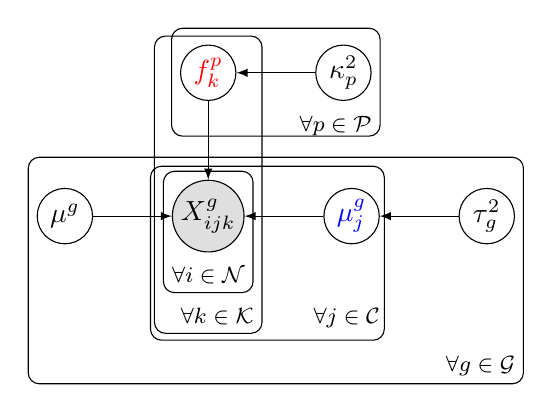
\begin{tikzpicture}
          \node[obs] (xgijk) {$X_{ijk}^{g}$};
          \node[latent, right=of xgijk] (mgj) {\myemph{$\mu_{j}^{g}$}};
          \node[latent, right=of mgj] (sgj) {$\tau_{g}^{2}$};
          \node[latent, above=of xgijk] (mk) {\mywarn{$f_{k}^{p}$}};
          \node[latent, right=of mk] (si) {$\kappa^{2}_{p}$};
          \node[latent, left=of xgijk] (mg) {$\mu^{g}$};

          \path[draw=black,->] (mgj) edge (xgijk);
          \path[draw=black,->] (sgj) edge (mgj);
          \path[draw=black,->] (mk) edge (xgijk);
          \path[draw=black,->] (si) edge (mk);
          \path[draw=black,->] (mg) edge (xgijk);
          
          \plate [inner sep=0.1cm, xshift=0.0cm]{plate0} {(xgijk)} {$\forall i \in \mathcal{N}$};
          \plate [inner sep=0.1cm, xshift=-0.05cm, yshift=-0.05cm] {plate1} {(plate0) (mgj)} {$\forall j\in \mathcal{C}$};
          \plate [inner sep=0.1cm, yshift=0.0cm] {plate2} {(plate0) (mk)} {$\forall k\in \mathcal{K}$};
          \plate [inner sep=0.1cm, yshift=0.0cm] {plate3} {(plate0) (plate1)
            (mg) (sgj)} {$\forall g\in \mathcal{G}$};
          \plate [inner sep=0.1cm, yshift=0.1cm] {plate4} { (si) (mk)}  {$\forall p \in \mathcal{P}$};
        \end{tikzpicture}
      }

\end{column}
\end{columns}
\vspace{0.5em}
$\kappa_{p}^{2}$ and $\tau_{g}^{2}$ are treated as the same as in the previous models. $\bm{B}_{G\times p} = {\{\bm{b}_{g=1},\bm{b}_{g=2},\ldots, 
  \bm{b}_{g=G}\}}_{g=1,\ldots,G}^{t}$, which describes the gene modules. For
example, each row $\bm{b}_{g=1}^{t}$ can be one-hot binary vector
describing which gene module the gene belongs to. We can also estimate B using
principle components (PCs) from principle component analysis (PCA) of the genes
on the cells.
\end{frame}

\subsection{mssc}
% \begin{frame}{Gene-wise individual effect}
  \(X_{ijk}^g\) represent the read count of the gene
  {\it g} on the cell {\it i} from the individual \mywarn{k}. \myemph{j} labels
  the group the individual \mywarn{k} belongs to. \(S_{ijk}\) represents the
  number of total counts in the cell {\it i} from the individual \mywarn{k}.
  \vspace{1em}
  \begin{columns}
    \begin{column}{0.5\textwidth}
      \begin{align*}
        X_{ijk}^{g} &\sim {\it Poisson} (S_{ijk}\cdot \lambda_{jk}^{g})\\
        \ln \lambda_{jk}^{g} &= \mu^{g} + \mywarn{\mu_{k}^{g}} + \myemph{\mu_{j}^{g}} \\
        \mu^{g} &\sim \mathcal{N}(0, \sigma^{2}_{0}) \\
        \mywarn{\mu_{k}^{g}} &\sim \mathcal{N}(0, \kappa^{2}_{g}) \\
        \myemph{\mu_{j}^{g}} &\sim \mathcal{N}(0, \tau^{2}_{g}) \\
        % \kappa^{2}_{g} &\sim invgamma(\alpha_{0}, \beta_{0}) \\
        % \tau^{2}_{g} &\sim invgamma(\alpha_{1}, \beta_{1})
      \end{align*}
    \end{column}
    \begin{column}{0.6\textwidth}
      \scalebox{0.85}{
        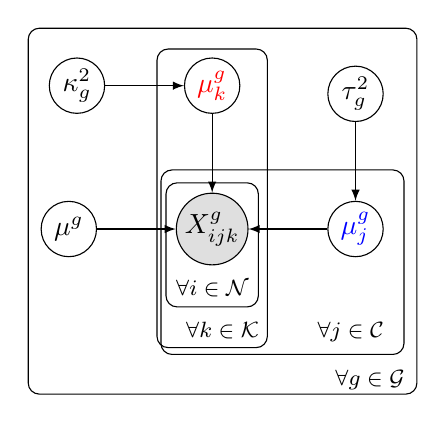
\begin{tikzpicture}
          \node[obs] (xgijk) {$X_{ijk}^{g}$};
          \node[latent, right=of xgijk] (mgj) {\myemph{$\mu_{j}^{g}$}};
          \node[latent, above=of mgj] (sgj) {$\tau_{g}^{2}$};
          \node[latent, above=of xgijk] (mk) {\mywarn{$\mu_{k}^{g}$}};
          \node[latent, left=of mk] (si) {$\kappa^{2}_{g}$};
          \node[latent, left=of xgijk] (mg) {$\mu^{g}$};

          \path[draw=black,->] (mgj) edge (xgijk);
          \path[draw=black,->] (sgj) edge (mgj);
          \path[draw=black,->] (mk) edge (xgijk);
          \path[draw=black,->] (si) edge (mk);
          \path[draw=black,->] (mg) edge (xgijk);
          
          \plate {plate0} {(xgijk)} {$\forall i \in \mathcal{N}$};
          \plate [inner sep=0.15cm, xshift=0.1cm] {plate1} {(plate0) (mgj)} {$\forall j\in \mathcal{C}$};
          \plate [inner sep=0.1cm, yshift=0.0cm]{plate2} {(plate0) (mk)} {$\forall k\in \mathcal{K}$};
          \plate [inner sep=0.15cm, yshift=0.1cm] {plate3} {(plate1) (plate2)
            (mk) (mg) (sgj)} {$\forall g\in \mathcal{G}$};
        \end{tikzpicture}
      }
    \end{column}
  \end{columns}
  $\kappa^{2}_{g}$ and $\tau^{2}_{g}$ have the priors of Inverse-Gamma distribution.
\end{frame}

% \begin{frame}{Hierarchical Bayesian Model}
  $\kappa^{2}_{g}$ and $\tau^{2}_{g}$ are
  estimated by the hierarchical structures shared among genes.
  \vspace{1em}
  \begin{columns}
    \begin{column}{0.5\textwidth}
      \begin{align*}
        X_{ijk}^{g} &\sim {\it Poisson} (S_{ijk}\cdot \lambda_{jk}^{g})\\
        \ln \lambda_{jk}^{g} &= \mu^{g} + \mywarn{\mu_{k}^{g}} + \myemph{\mu_{j}^{g}} \\
        \mu^{g} &\sim \mathcal{N}(0, \sigma^{2}_{0}) \\
        \mywarn{\mu_{k}^{g}} &\sim \mathcal{N}(0, \kappa^{2}_{g}) \\
        \myemph{\mu_{j}^{g}} &\sim \mathcal{N}(0, \tau^{2}_{g}) \\
        \kappa^{2}_{g} &\sim invgamma(\alpha_{\kappa}, \beta_{\kappa}) \\
        \tau^{2}_{g} &\sim invgamma(\alpha_{\tau}, \beta_{\tau}) \\
        % \mu_{ind}^{g} &\sim \mathcal{N}(\mu_{ind_{0}}, \sigma_{ind_{0}}^{2}) \\
        % \sigma_{g,ind}^{2} &\sim invgamma(alpha_{1}, beta_{1}) \\
        % \mu &\sim \mathcal{N}(\mu_{0}, \sigma_{0}^{2}) \\
        % \sigma^{2} &\sim invgamma(alpha_{0}, beta{0})
      \end{align*}
    \end{column}
    \begin{column}{0.6\textwidth}
      \scalebox{0.85}{
        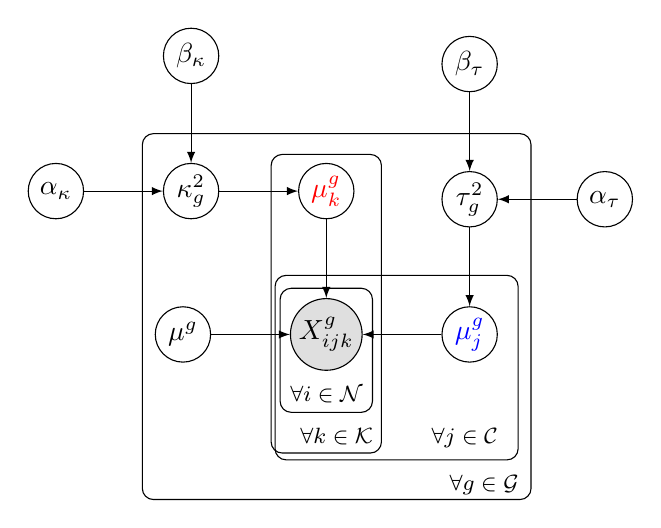
\begin{tikzpicture}
          \node[obs] (xgijk) {$X_{ijk}^{g}$};
          \node[latent, right=of xgijk] (mgj) {\myemph{$\mu_{j}^{g}$}};
          \node[latent, above=of mgj] (sgj) {$\tau_{g}^{2}$};
          \node[latent, right=of sgj] (aj) {$\alpha_{\tau}$};
          \node[latent, above=of sgj] (bj) {$\beta_{\tau}$};
          \node[latent, above=of xgijk] (mk) {\mywarn{$\mu_{k}^{g}$}};
          \node[latent, left=of mk] (si) {$\kappa^{2}_{g}$};
          \node[latent, left=of si] (ak) {$\alpha_{\kappa}$};
          \node[latent, above=of si]  (bk) {$\beta_{\kappa}$};
          \node[latent, left=of xgijk] (mg) {$\mu^{g}$};

          \path[draw=black,->] (mgj) edge (xgijk);
          \path[draw=black,->] (sgj) edge (mgj);
          \path[draw=black,->] (aj) edge (sgj);
          \path[draw=black,->] (bj) edge (sgj);
          \path[draw=black,->] (mk) edge (xgijk);
          
          \path[draw=black,->] (si) edge (mk);
          \path[draw=black,->] (ak) edge (si);
          \path[draw=black,->] (bk) edge (si);
          \path[draw=black,->] (mg) edge (xgijk);
          
          \plate {plate0} {(xgijk)} {$\forall i \in \mathcal{N}$};
          \plate [inner sep=0.15cm, xshift=0.1cm] {plate1} {(plate0) (mgj)} {$\forall j\in \mathcal{C}$};
          \plate [inner sep=0.1cm, yshift=0.0cm]{plate2} {(plate0) (mk)} {$\forall k\in \mathcal{K}$};
          \plate [inner sep=0.15cm, yshift=0.1cm] {plate3} {(plate1) (plate2) (mg) } {$\forall g\in\mathcal{G}$};
        \end{tikzpicture}
      }
    \end{column}
  \end{columns}
  $\alpha_{\kappa}$, $\beta_{\kappa}$, $\alpha_{\tau}$ and $\beta_{\tau}$ have the
  priors of Gamma distribution.
\end{frame}

% \begin{frame}
  Furthermore, we model individual batch effects on the \mywarn{gene modules},
  instead of shared among the genes or independent on every gene.
  \begin{columns}
    \begin{column}{0.5\textwidth}
\begin{align*}
  X_{ijk}^{g} &\sim {\it Poisson} (S_{ijk}\cdot \lambda_{jk}^{g})\\
  \ln \lambda_{jk}^{g} &= \mu^{g} + \mywarn{\mu_{k}^{g}} + \myemph{\mu_{j}^{g}} \\
  \mu^{g} &\sim \mathcal{N}(0, \sigma^{2}_{0}) \\
  \mywarn{\mu_{k}^{g}} &= \bm{b}_{g}^{t}\cdot \mywarn{\bm{f}_{k}},~~\bm{b}_{g},\bm{f}_{k}\in \mathcal{R}^{p\times 1}\\
  \mywarn{f_{k}^{p}} &\sim \mathcal{N}(0, \kappa^{2}_{p}) \\
  \myemph{\mu_{j}^{g}} &\sim \mathcal{N}(0,\tau^{2}_{g})
\end{align*}
\end{column}
\begin{column}{0.6\textwidth}
      \scalebox{0.85}{
        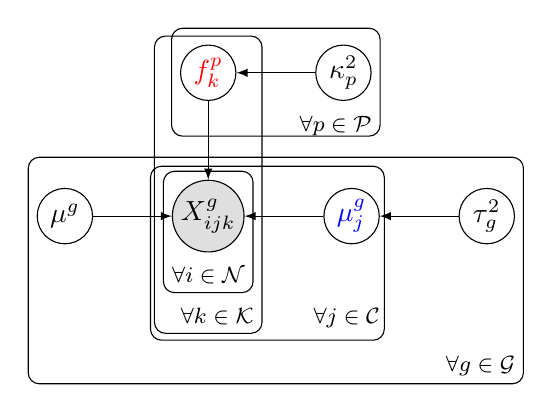
\begin{tikzpicture}
          \node[obs] (xgijk) {$X_{ijk}^{g}$};
          \node[latent, right=of xgijk] (mgj) {\myemph{$\mu_{j}^{g}$}};
          \node[latent, right=of mgj] (sgj) {$\tau_{g}^{2}$};
          \node[latent, above=of xgijk] (mk) {\mywarn{$f_{k}^{p}$}};
          \node[latent, right=of mk] (si) {$\kappa^{2}_{p}$};
          \node[latent, left=of xgijk] (mg) {$\mu^{g}$};

          \path[draw=black,->] (mgj) edge (xgijk);
          \path[draw=black,->] (sgj) edge (mgj);
          \path[draw=black,->] (mk) edge (xgijk);
          \path[draw=black,->] (si) edge (mk);
          \path[draw=black,->] (mg) edge (xgijk);
          
          \plate [inner sep=0.1cm, xshift=0.0cm]{plate0} {(xgijk)} {$\forall i \in \mathcal{N}$};
          \plate [inner sep=0.1cm, xshift=-0.05cm, yshift=-0.05cm] {plate1} {(plate0) (mgj)} {$\forall j\in \mathcal{C}$};
          \plate [inner sep=0.1cm, yshift=0.0cm] {plate2} {(plate0) (mk)} {$\forall k\in \mathcal{K}$};
          \plate [inner sep=0.1cm, yshift=0.0cm] {plate3} {(plate0) (plate1)
            (mg) (sgj)} {$\forall g\in \mathcal{G}$};
          \plate [inner sep=0.1cm, yshift=0.1cm] {plate4} { (si) (mk)}  {$\forall p \in \mathcal{P}$};
        \end{tikzpicture}
      }

\end{column}
\end{columns}
\vspace{0.5em}
$\kappa_{p}^{2}$ and $\tau_{g}^{2}$ are treated as the same as in the previous models. $\bm{B}_{G\times p} = {\{\bm{b}_{g=1},\bm{b}_{g=2},\ldots, 
  \bm{b}_{g=G}\}}_{g=1,\ldots,G}^{t}$, which describes the gene modules. For
example, each row $\bm{b}_{g=1}^{t}$ can be one-hot binary vector
describing which gene module the gene belongs to. We can also estimate B using
principle components (PCs) from principle component analysis (PCA) of the genes
on the cells.
\end{frame}

\begin{frame}{Negative Binomial Generalized Linear Model}
  Let \(X_{ij}\) represent the UMI counts for the gene \(i\) in the cell \(j\)
  \begin{align}
    X_{ij} &\sim NB(\mu_{ij}, \phi_i) \\
    \mu_{ij}  &= S_j * \lambda_{ij} \\
    \log(\lambda_{ij})  &= \sum_r d_{jr} \beta_{ir} \\
    \phi_{i} &\sim Gamma(\alpha_0, \beta_0) 
  \end{align}
  \begin{equation*}
    \resizebox{0.6\hsize}{!}{$%
    \bm{\beta_r} \sim {\cal N}\left(\bm{0}, 
    \begin{bmatrix}
      \sigma_0^2  &     & & & &\\
      &   \myemph{\sigma_{ind}^2} & & & &\\
      &    &     \ddots &      & & \\
      &    &     & \myemph{\sigma_{ind}^2}  & & \\
      &    &     &  &   \mywarn{\sigma_{cond}^2} &  \\
      &    &     &   &    &  \mywarn{\sigma_{cond}^2} 
      \end{bmatrix}
    \right)
    $%
    }%
  \end{equation*}
  \begin{equation*}
    \mathbf{d_j} = \left(1, \overbrace{(0, \myemph{1}, \dots, 0, 0)}, \underbrace{(\mywarn{1}, 0)}\right)
  \end{equation*}

\end{frame}

\begin{frame}
  \begin{figure}
    \centering
    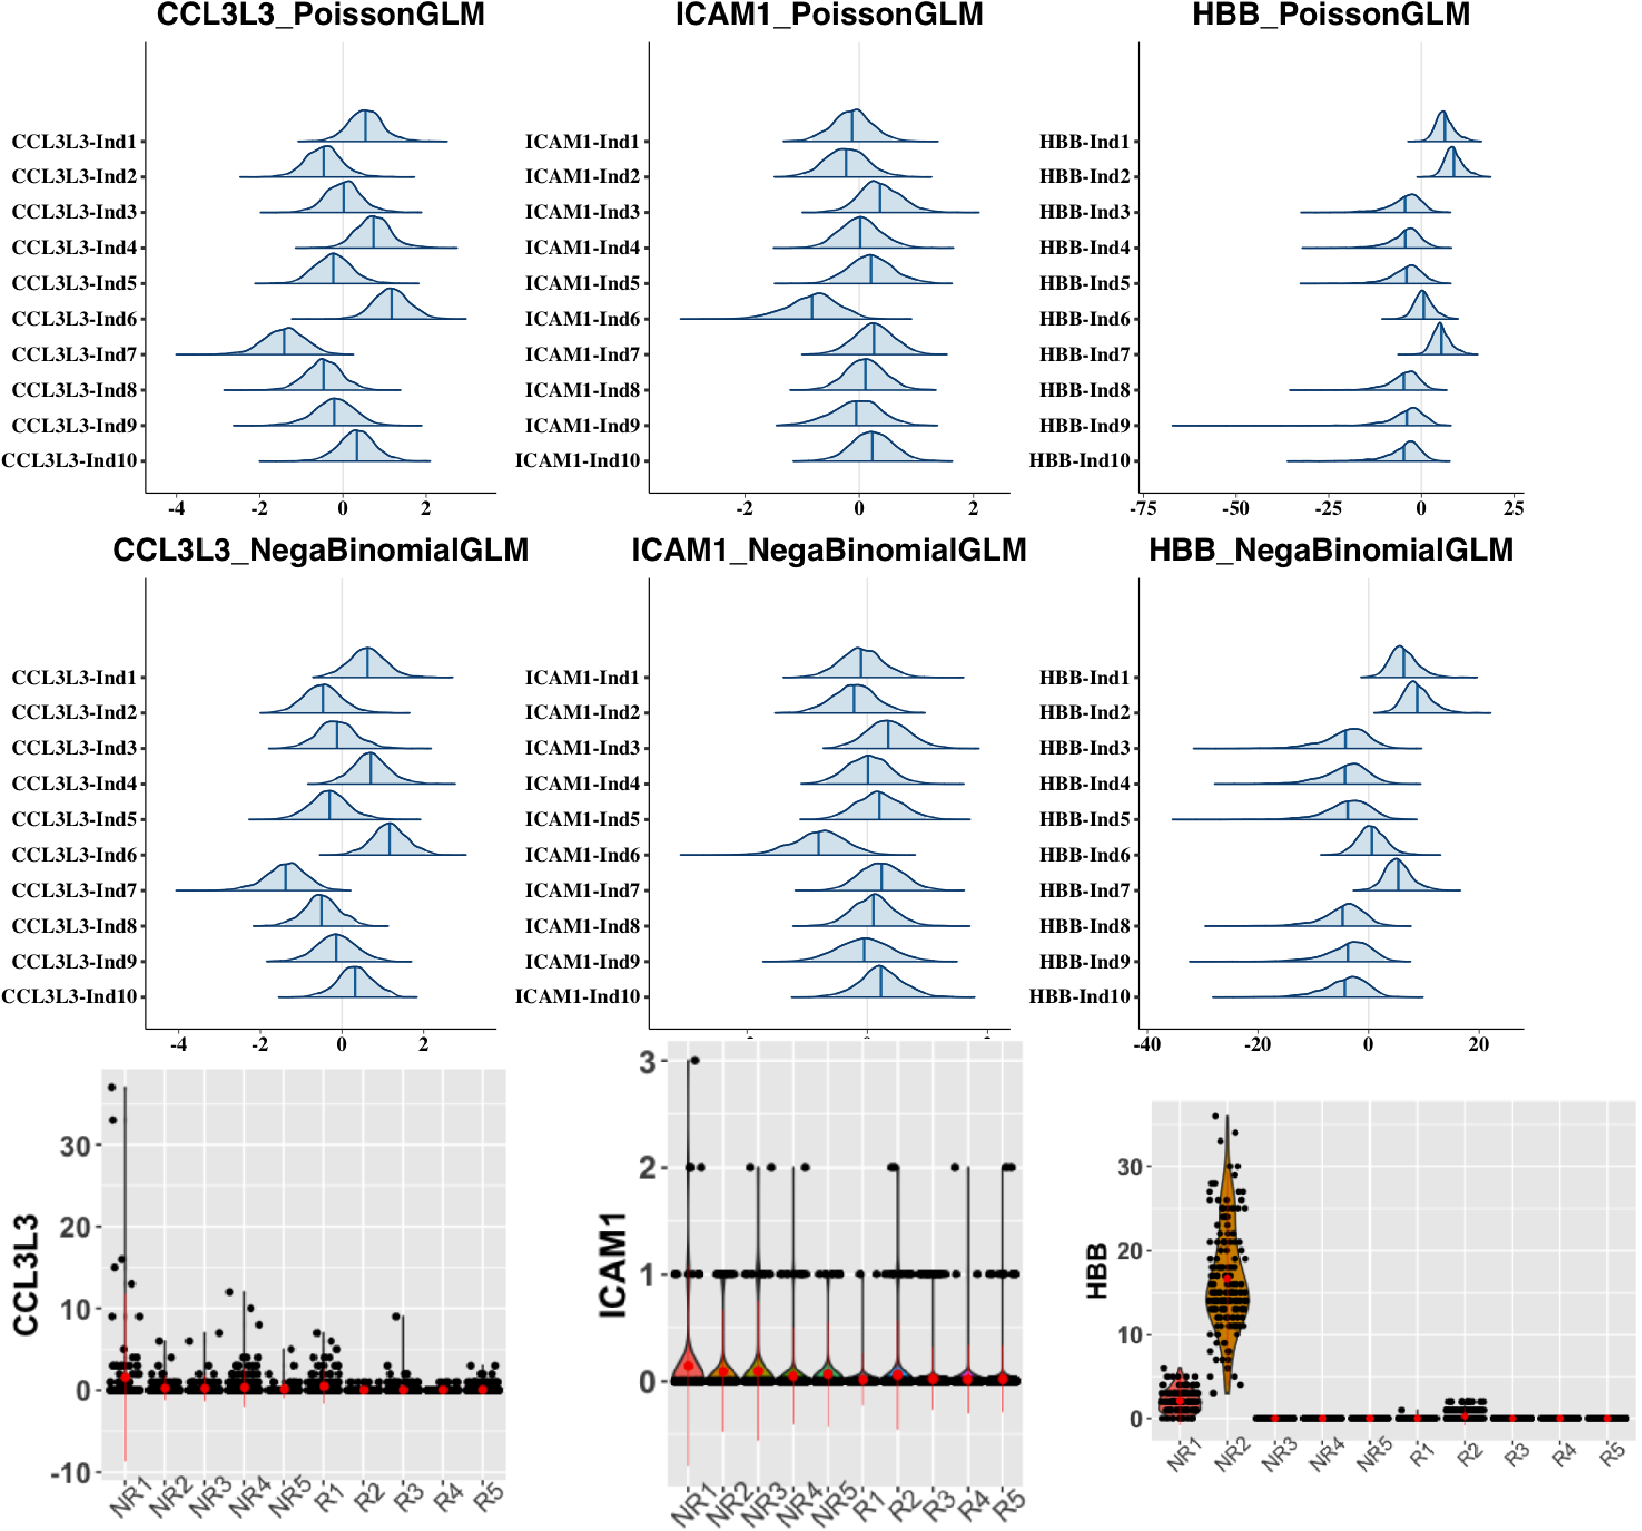
\includegraphics[height = \textheight]{poi_nb_pbmc_inds}
  \end{figure}
\end{frame}

\begin{frame}
  \begin{figure}
    \centering
    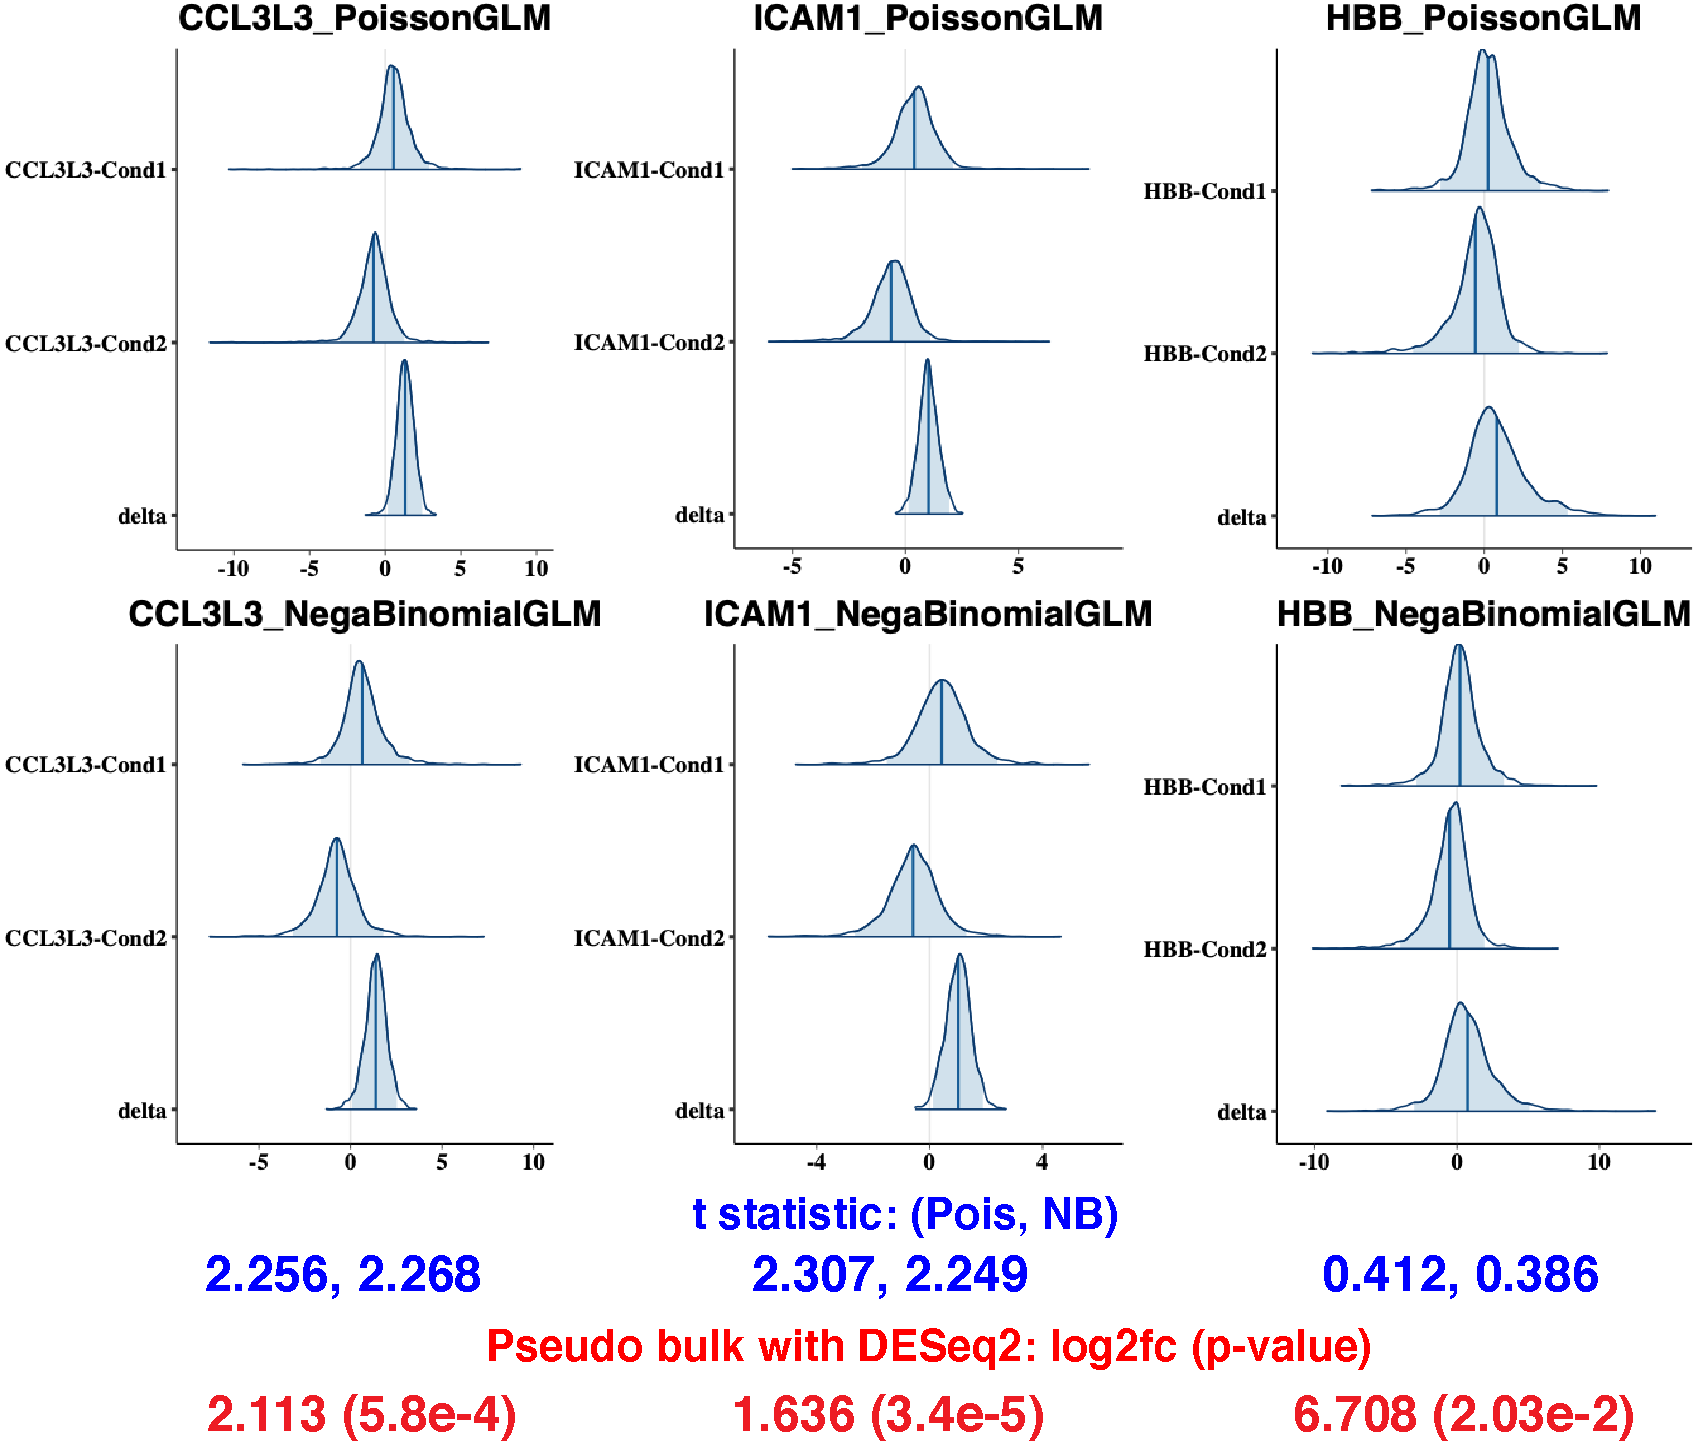
\includegraphics[height = \textheight]{poi_nb_pbmc_conds_with_scores}
  \end{figure}
\end{frame}

\section{Simulation}
\subsection{SymSim}
\begin{frame}
  \begin{figure}
    \centering
    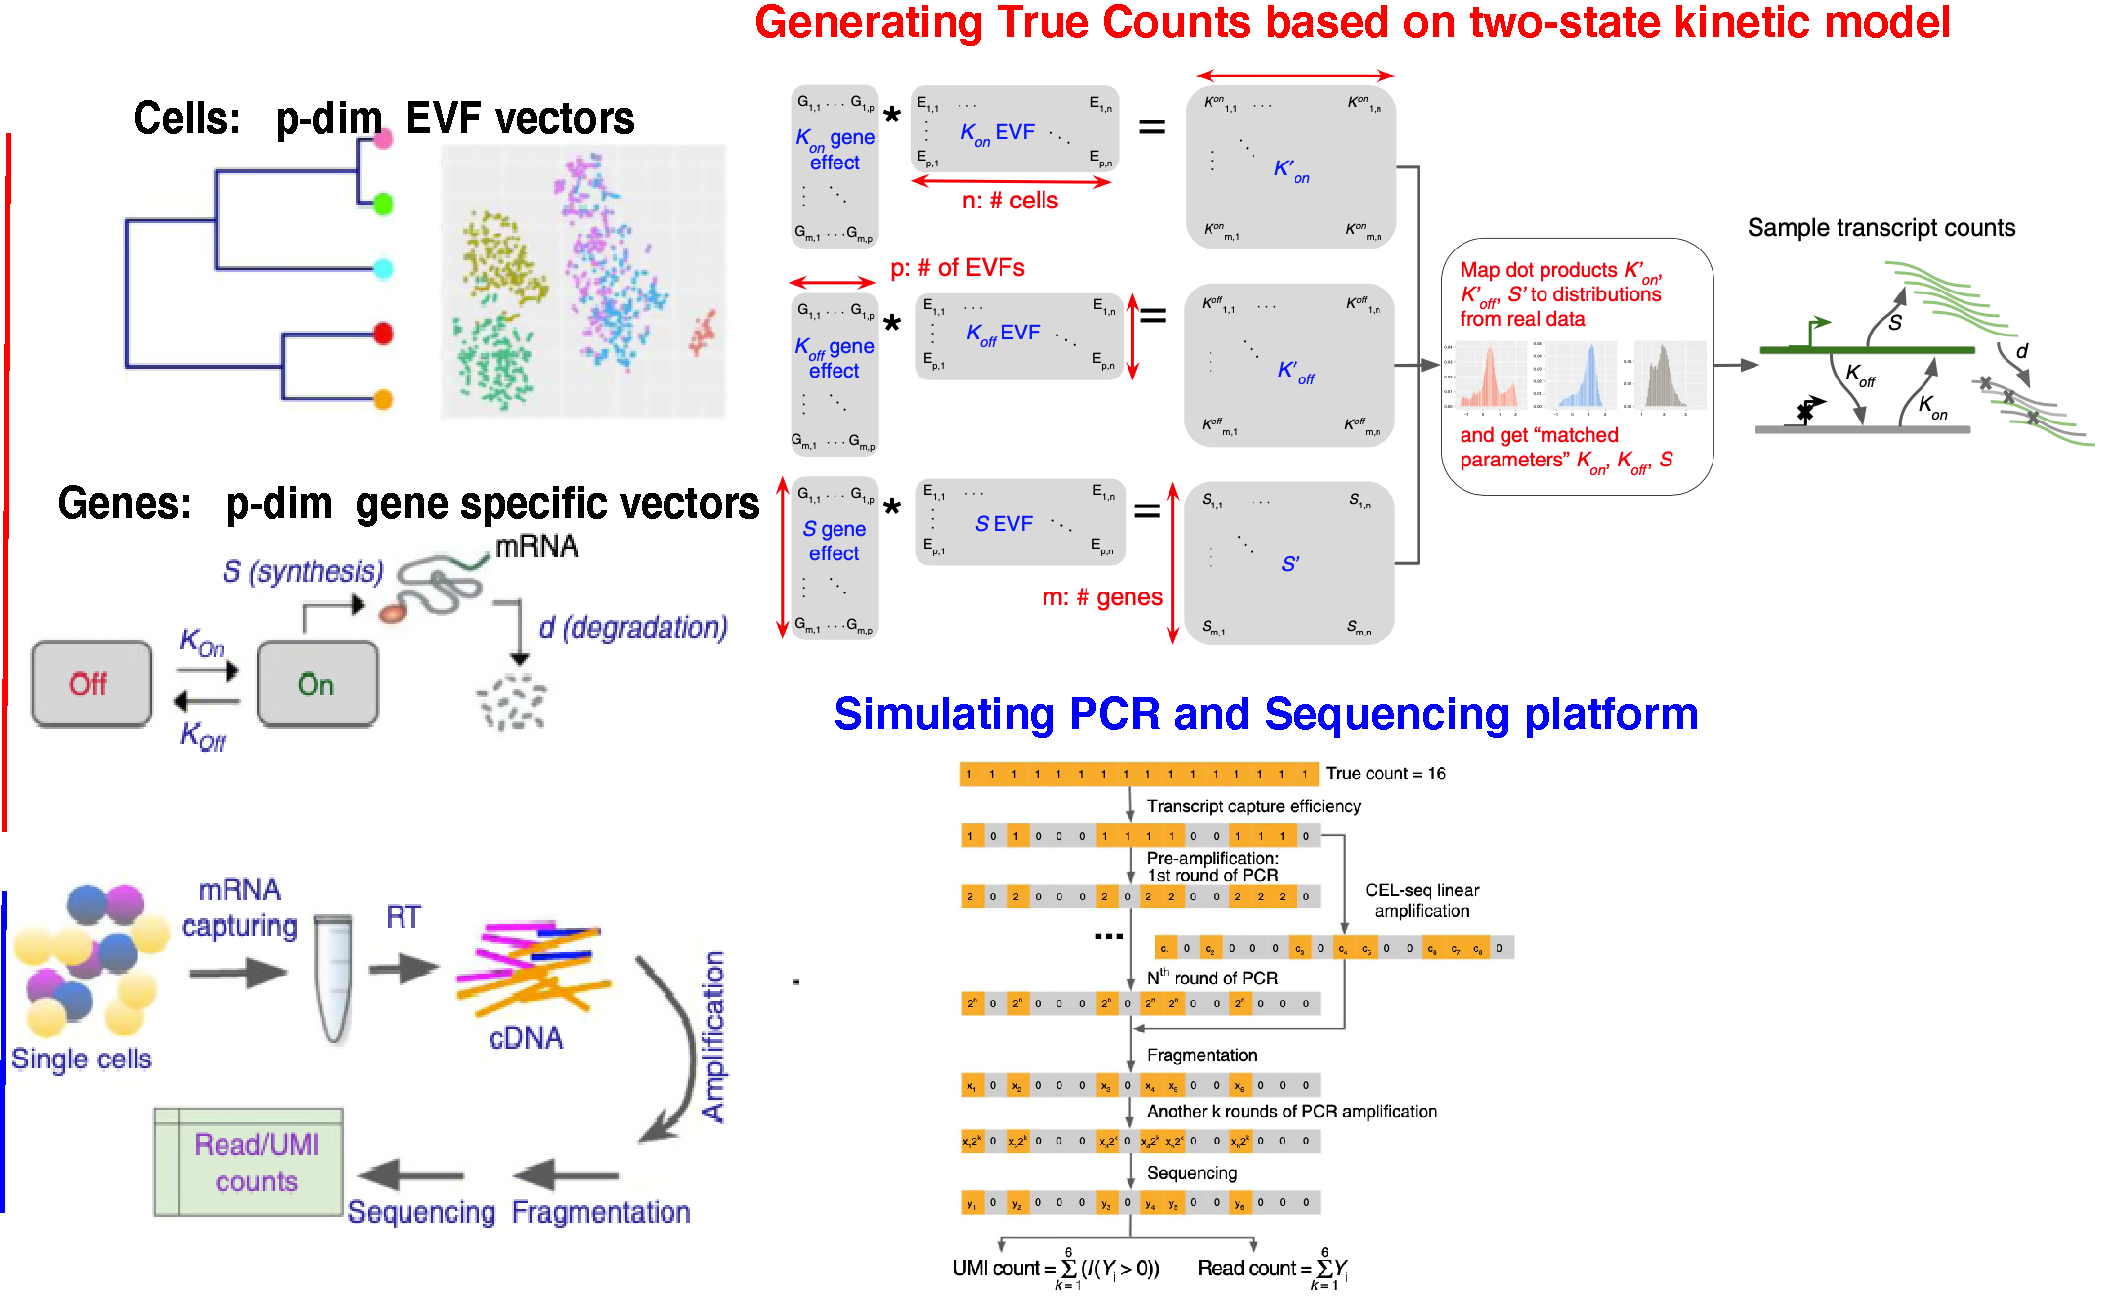
\includegraphics[width=\textwidth]{mssc-symsim}
    \caption{SymSim Overview (\cite{zhang2019simulating})}
  \end{figure}
\end{frame}

\begin{frame}
  \begin{figure}
    \centering
    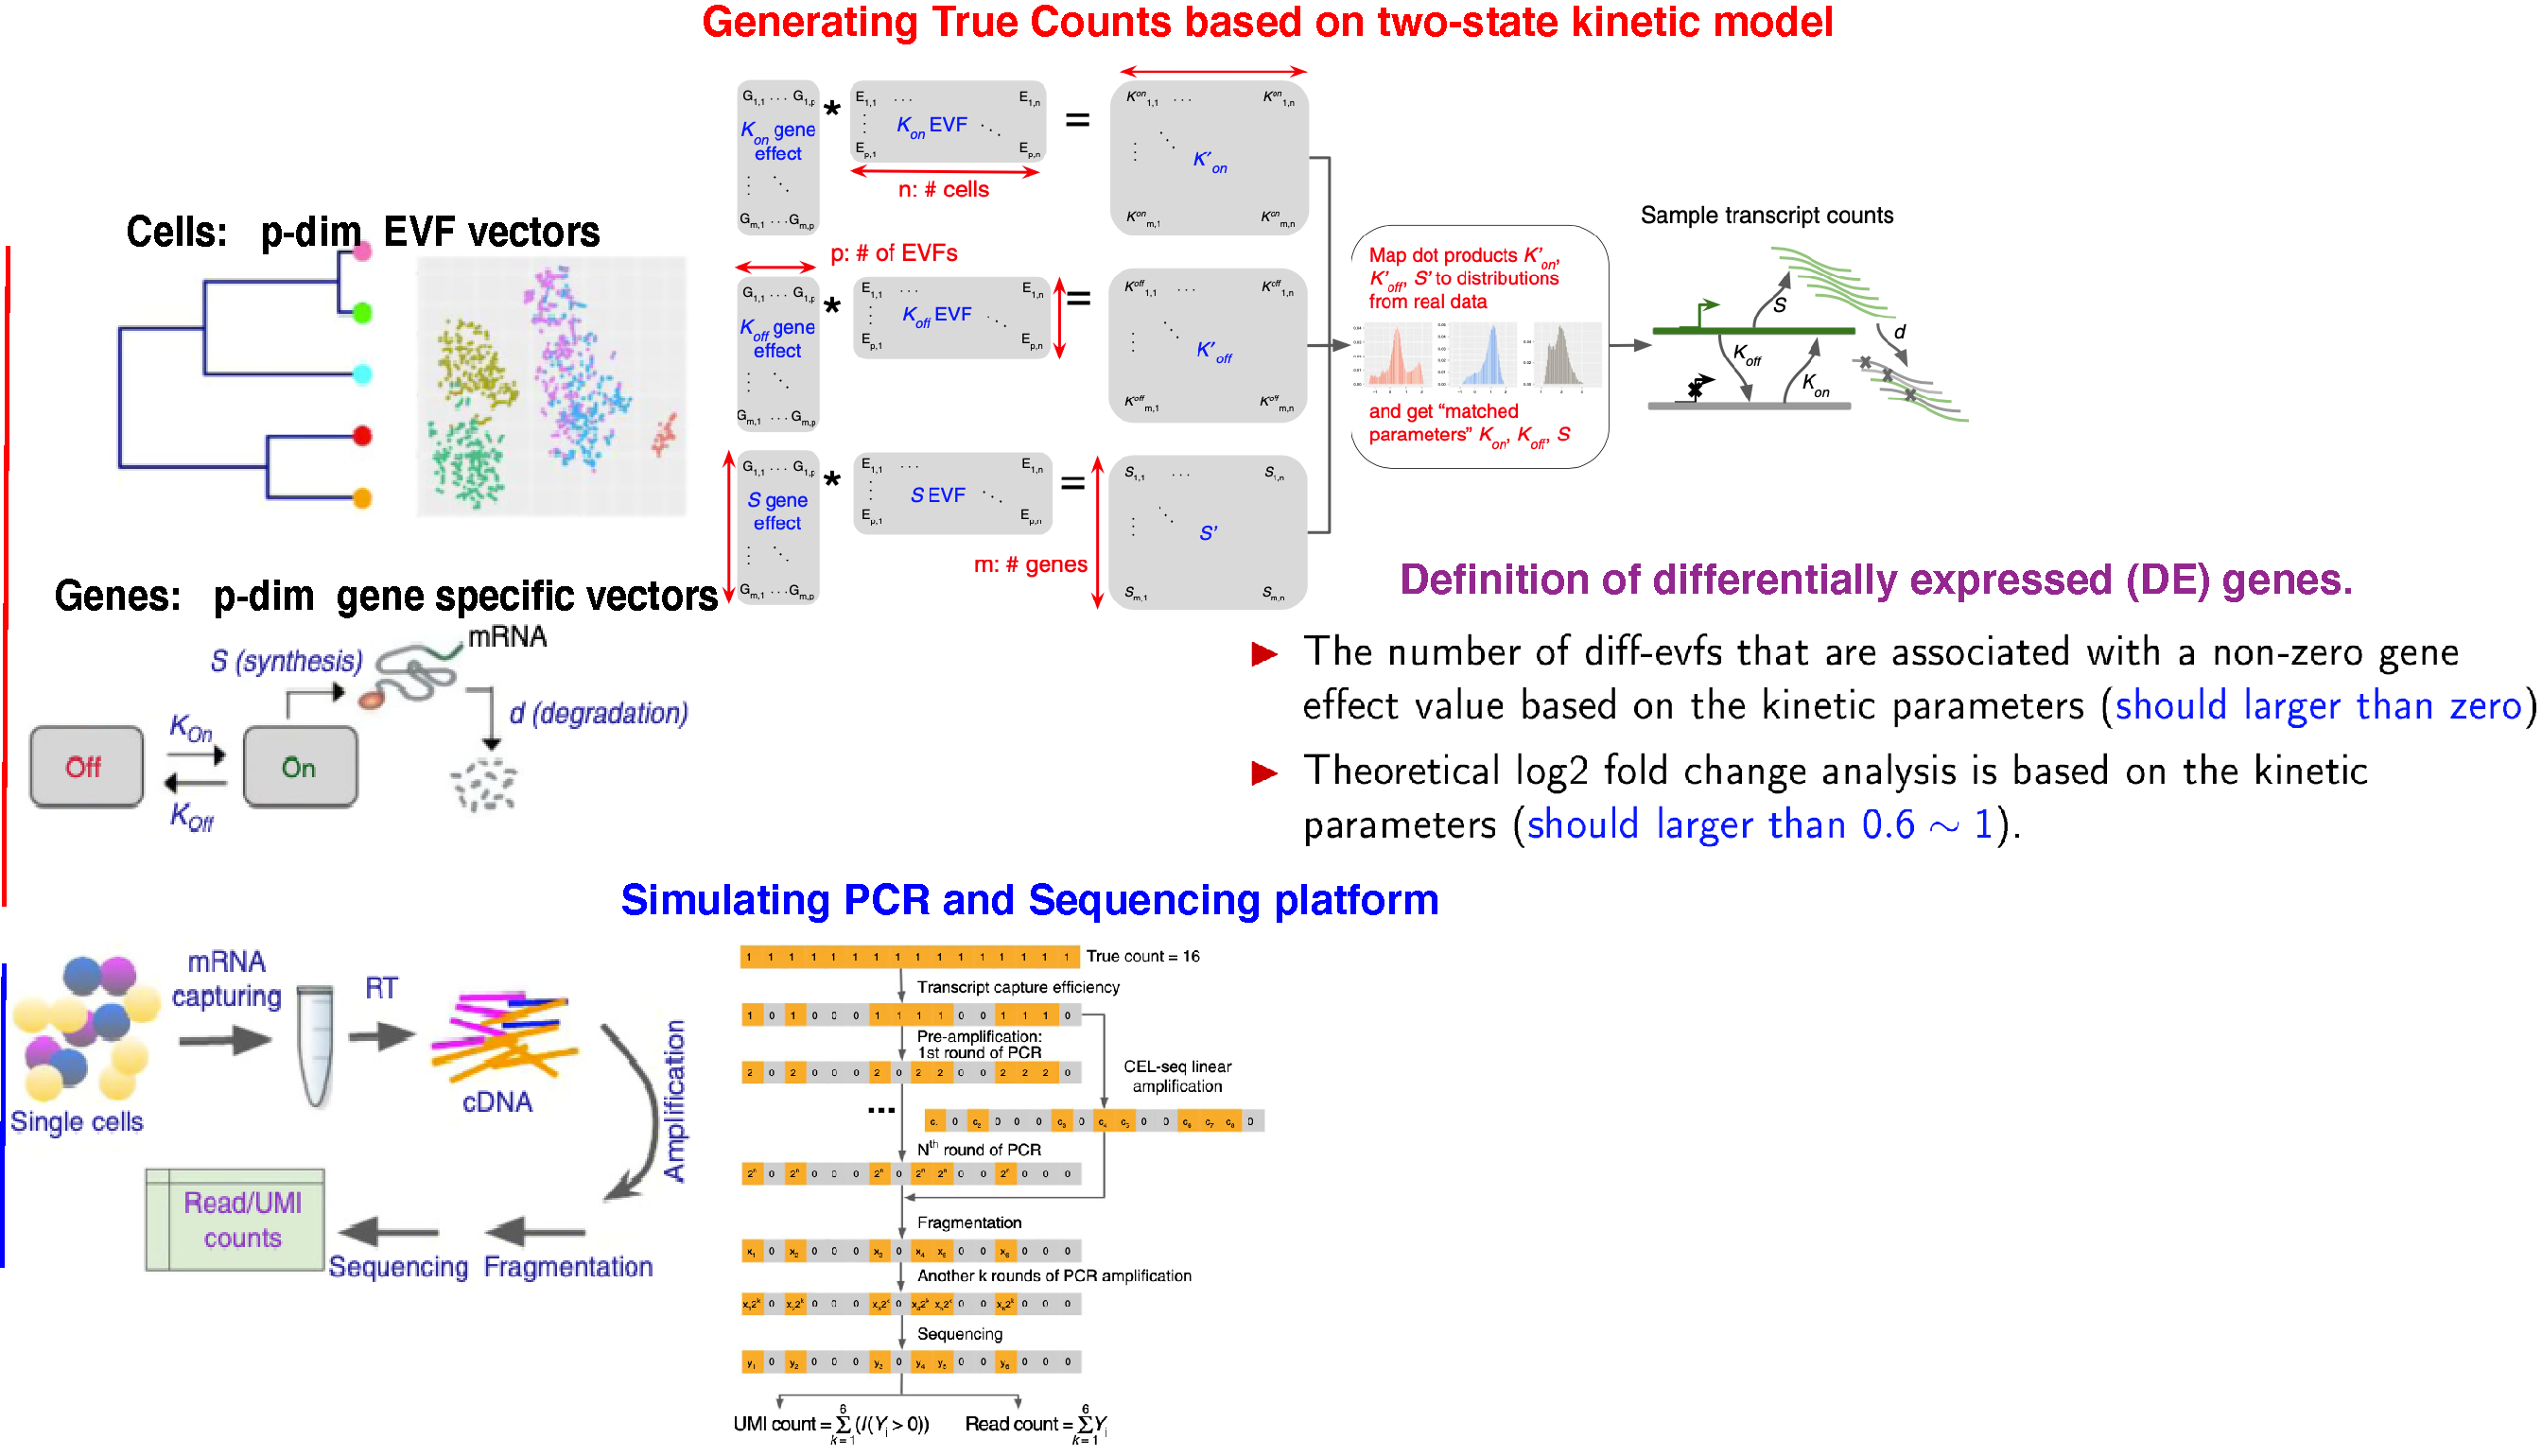
\includegraphics[width=\textwidth]{mssc-symsim_diffgene}
    \caption{DE analysis in SymSim}
  \end{figure}
\end{frame}

\begin{frame}
  \begin{figure}
    \centering
    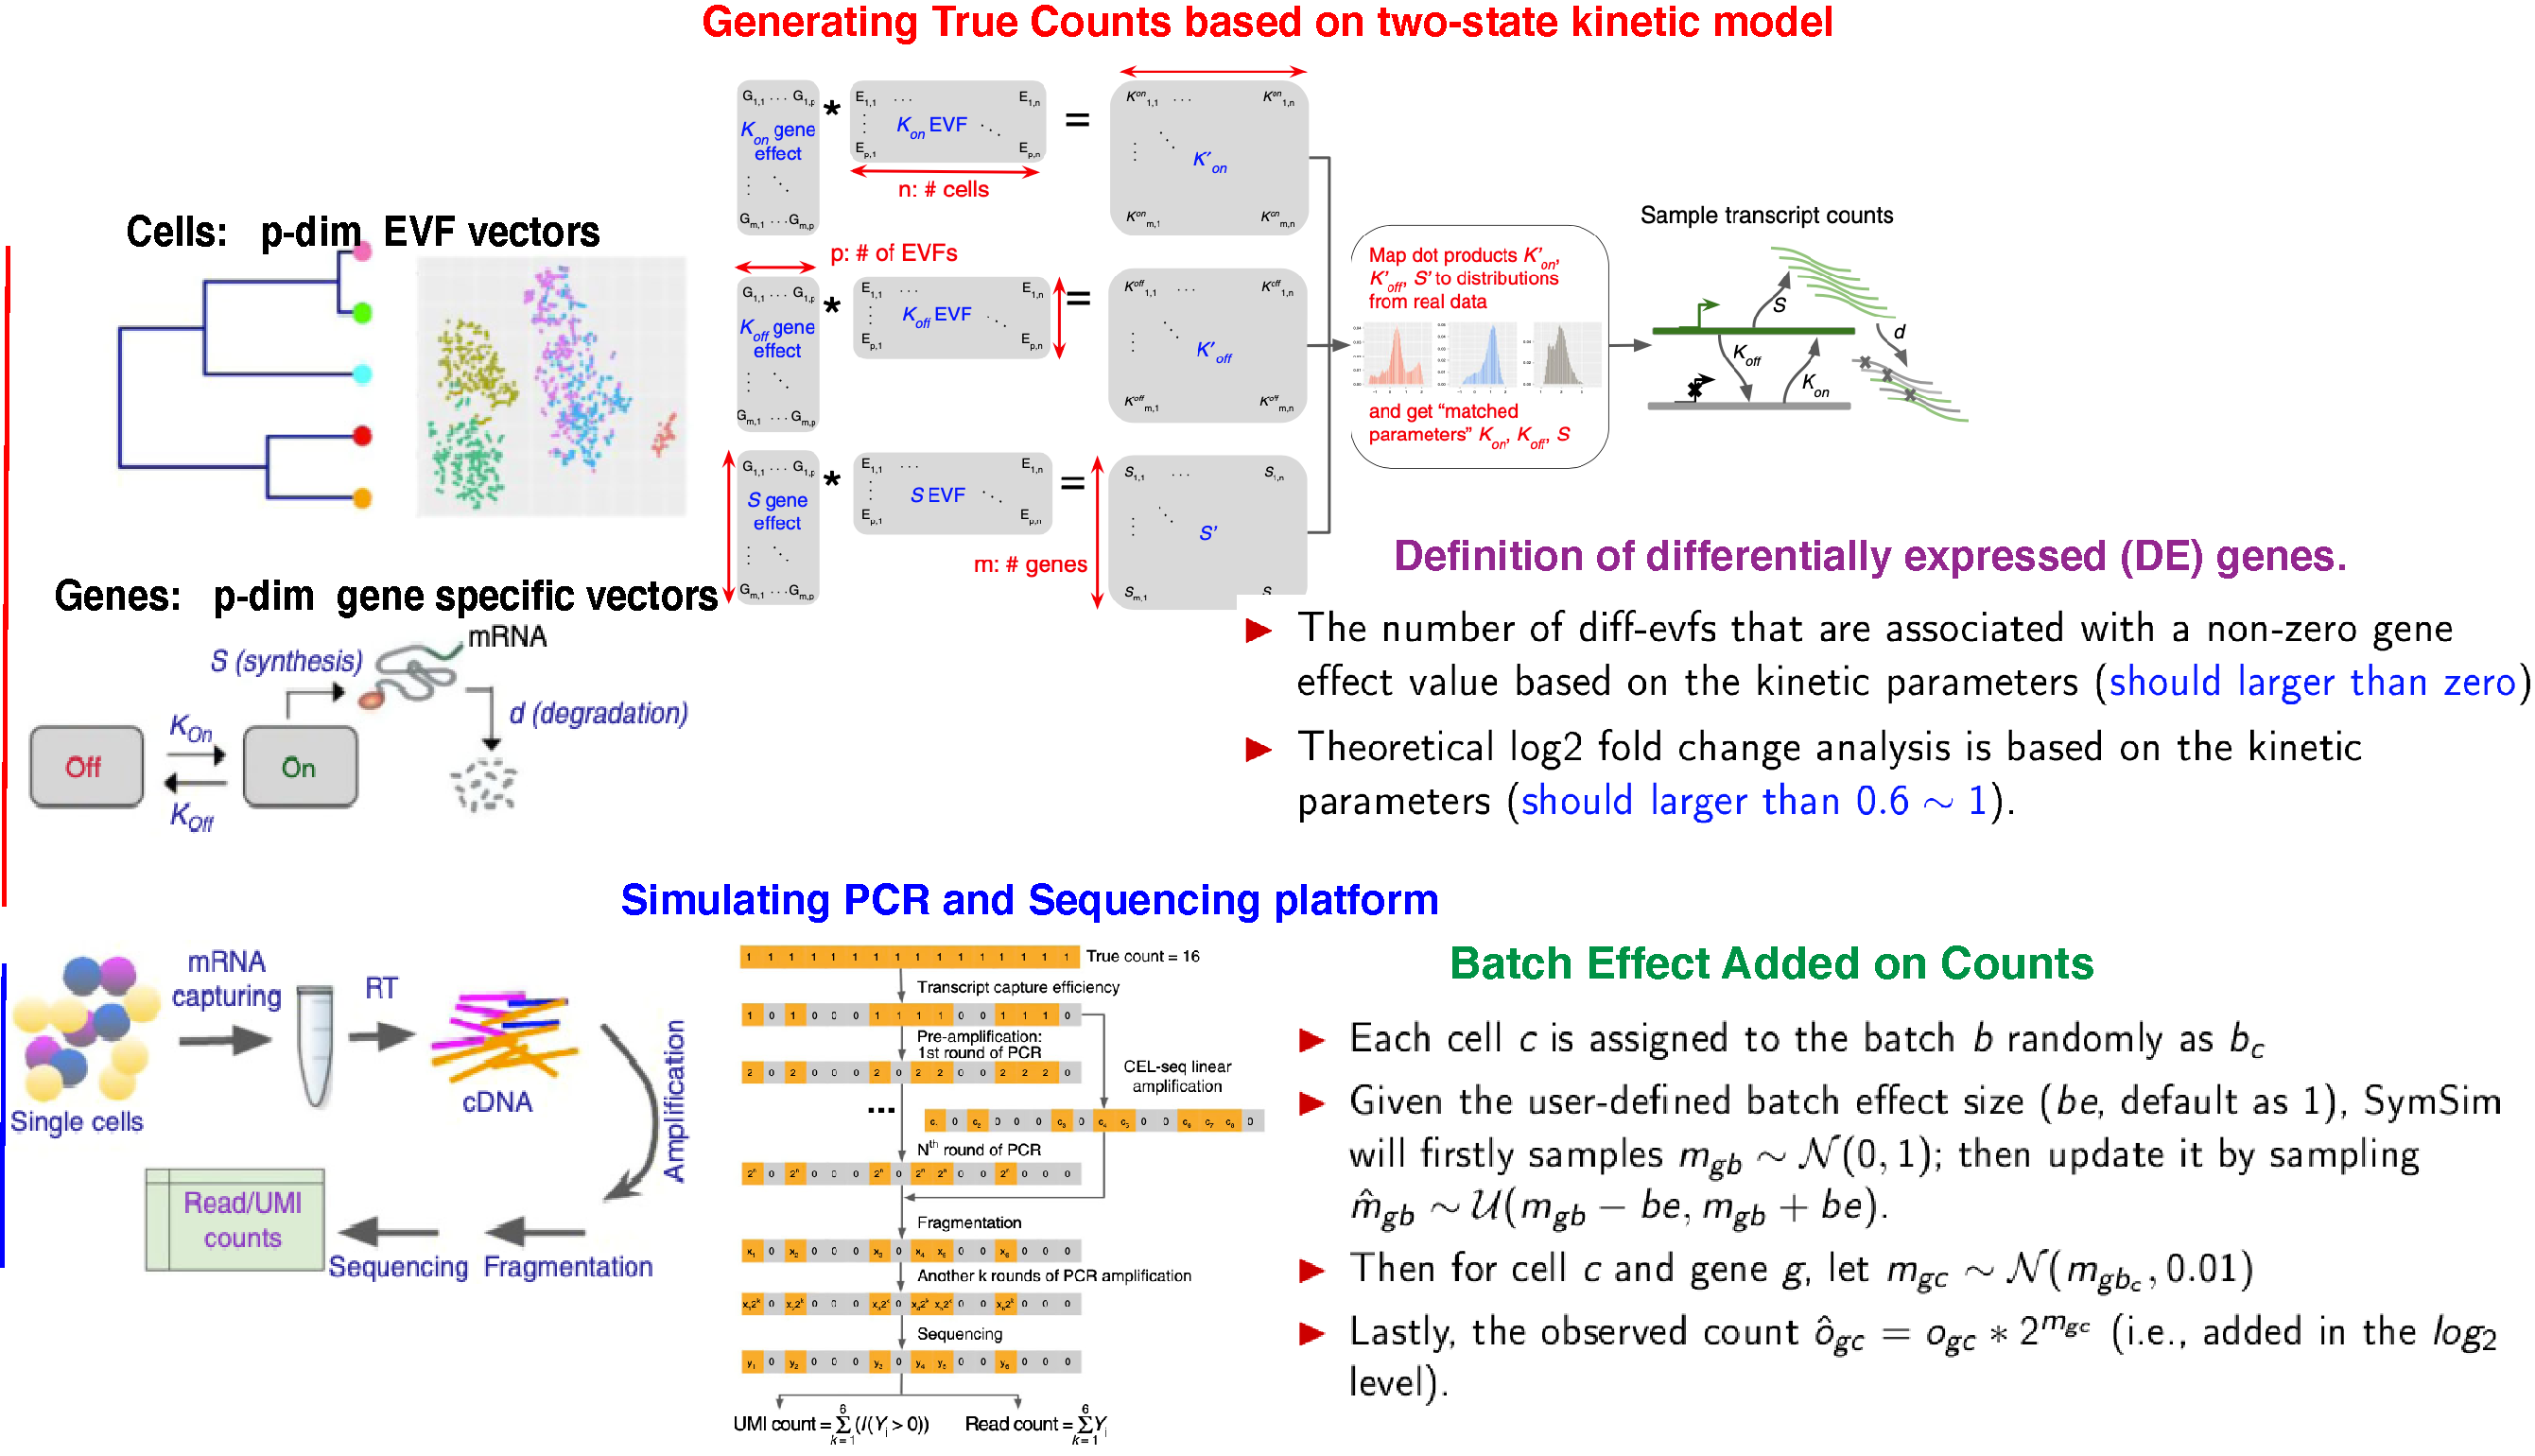
\includegraphics[width=\textwidth]{mssc-symsim_batcheffect}
    \caption{Batch effect in SymSim}
  \end{figure}
\end{frame}

\subsection*{MSSC SymSim}
\begin{frame}
  \frametitle{Simulation based on SymSim}
  \begin{itemize}
  \item
    2000 cells, 300 genes, 10 batch (individuals)
    \begin{itemize}
    \item
      Each individual (ind): about 200 cells
    \item
      \mywarn{Condition 1: Ind 1 to 5 } {\it v.s.} \myemph{Condition 2: Ind 6 to 10}
    \item
      Use the \myemph{two-leaf} phylo-tree, which lets SymSim to generate two cell populations
      as one cell type in two conditions in MSSC.
    \item
      1000 cells in each condition
    \end{itemize}
  \item
    Batch effect added in two sequential steps:
    \begin{enumerate}
    \item
      The default SymSim strategy to add both gene and
      individual-specific batch effect.
    \item
      Sample some non-differential expressed genes, add strong batch effect
      sizes for 1, 2 and 6 to simulate the biased response. {\it For
        instance, in our simulation, \mywarn{71} DE genes, and \mywarn{34}
      \myemph{strictly} non-DE genes. We sample \mywarn{20} genes from the
      strictly non-DE genes in the second step.} 
    \end{enumerate}
  \end{itemize}
\end{frame}

\begin{frame}
  \frametitle{DE genes when no batch effect}
  \begin{figure}
    \centering
    \includegraphics[width=\textwidth]{sample_umi_deg_1}
    \caption{Before batch effect: DE genes} 
  \end{figure}
\end{frame}

\begin{frame}
  \frametitle{non-DE genes when no batch effect}
  \begin{figure}
    \centering
    \includegraphics[width=\textwidth]{sample_umi_ndeg_1}
    \caption{Before batch effect: non-DE genes} 
  \end{figure}
\end{frame}

\begin{frame}
  \frametitle{DE genes after the first batch effect}
  \begin{figure}
    \centering
    \includegraphics[width=\textwidth]{sample_be_deg_1}
    \caption{First batch effect: DE genes} 
  \end{figure}
\end{frame}

\begin{frame}
  \frametitle{Non-DE genes after the first batch effect}
  \begin{figure}
    \centering
    \includegraphics[width=\textwidth]{sample_be_ndeg_1}
    \caption{First batch effect: non-DE genes} 
  \end{figure}
\end{frame}

\begin{frame}
  \frametitle{DE genes after the second batch effect}
  \begin{figure}
    \centering
    \includegraphics[width=\textwidth]{sample_2be_deg_1}
    \caption{Second batch effect: DE genes} 
  \end{figure}
\end{frame}

\begin{frame}
  \frametitle{Non-DE genes after the second batch effect}
  \begin{figure}
    \centering
    \includegraphics[width=\textwidth]{sample_2be_ndeg_1}
    \caption{Second batch effect: non-DE genes} 
  \end{figure}
\end{frame}

\subsection*{Gene-wise batch effect model}
\begin{frame}
  \frametitle{Result Summary based on the AUC}
  \begin{itemize}
  \item
    Both MCMC and VI shows almost the same result.
  \item
    Model v1-1 and v1-2 shows almost the same result, but v1-2 is more
    robustness than v1-1.
  \item
    On the simulation data set, pseudobulk is better than mssc (0.75 vs 0.72). 
  \end{itemize}
\end{frame}

\begin{frame}{Posterior t statistics vs p-value from DESeq2}
  \begin{figure}
    \centering
    \includegraphics[width=\textwidth]{p_v1-1_deg}
    \caption{DE genes: mssc vs pseudo} 
  \end{figure}
\end{frame}

\begin{frame}{Posterior t statistics vs p-value from DESeq2}
  \begin{figure}
    \centering
    \includegraphics[width=\textwidth]{p_v1-1_ndeg}
    \caption{Non-DE genes: mssc vs pseudo}
  \end{figure}
\end{frame}

\section{Real data}
\subsection{A simplified real case}
\begin{frame}
  \frametitle{DataSet}
  \begin{itemize}
  \item
    UMI-based scRNAseq Data: 5 cases vs. 5 controls
    \begin{itemize}
    \item
      In total, 26,000 cells (over 2,000 cells / individual).
    \item
      Identify cell types: using \myemph{Harmony}; choose cluster 2, which is
      cytotoxic T-cells, with 3,885 cells.
    \end{itemize}
  \item
    Select 27 genes from both top-ranked and low-ranked genes based on pseudo
    bulk analysis with \myemph{DESeq2}.
    \begin{itemize}
    \item
      Gene modules by hierarchical clustering of genes
      on cluster 2.
    \begin{itemize}
    \item
      Group1: ICAM1(DESeq2 Rank 6), XCL2 (DESeq2 Rank 13), XCL1 (DESeq2 Rank 43)
    \item
      Group2: RPS26P11 (DESeq2 Rank 15), LOC101929876 (DESeq2 Rank 22),LOC100996747 (DESeq2 Rank 97)
    \item
      Group3: HBA1 (DESeq2 Rank 14), HBA2, HBB, HBD 
    \item
      Group4: CCL3L3 (DESeq2 Rank 99), CCL3L1 (DESeq2 Rank 102), CCL3
    \end{itemize}
  \item
    Top-ranked genes: SNHG16,OASL,NAMPT,NFKB1,BCL2L11,IRF8,TPM4,TRAF4
  \item
    Low-ranked genes: KDM6A,ZNF721,HDDC2,YIPF5,MAK16, TOX
    \end{itemize}
  \end{itemize}
\end{frame}

\begin{frame}
\begin{figure}
  \centering
  \includegraphics[height = \textheight]{gene-module-clust2.pdf}
\end{figure}
\end{frame}

\begin{frame}
  \begin{figure}
    \centering
    \includegraphics[width = \textwidth]{GoldGenes.pdf}
  \end{figure}
\end{frame}

\subsubsection{Gene-wise individual effect}
\begin{frame}
  \begin{figure}
    \centering
    \includegraphics[height= \textheight]{v11-vs-v12-DE.pdf}
  \end{figure}
\end{frame}
\subsubsection{Gene-module individual effect}
\begin{frame}
  \begin{figure}
    \centering
    \includegraphics[height = \textheight]{v21-vs-v22-DE.pdf}
  \end{figure}
\end{frame}

\section{Discussion}
\subsection*{Simulation}
\begin{frame}
  \frametitle{Simulation limitations}
  \begin{itemize}
  \item
    Simulation: current batch effect is added \mywarn{after count generation}, while in
    our model, we model batch effects on \myemph{gene expression level}.
  \item
    Gene modules: batch effect estimation might be hard. So how about consider
    two gene modules: one is for the false positive ones, and the other is for
    the positive ones. Then let each of them share the same batch effect. And we
    estimate the batch effect on gene-module level.
  \item
    Pseudobulk analysis might over estimate the genes if the genes have lots of zero
    counts.
  \end{itemize}
\end{frame}

\section*{Supplementary}
\subsection*{Modeling scRNA-seq data}
\begin{frame}
  \frametitle{Droplet scRNAseq is not zero-inflated \cite{svensson2020droplet}}
  \begin{itemize}
  \item
    The original "dropout" problem of yielding an inflation of zero values
    in scRNA-seq data was in the description of single-cell differential
    expression (SCDE) \cite{kharchenko2014bayesian}, which was on low-throughput
    plate-based methods, like Smart-seq and STRT-seq.
  \item
    Investigate the number of zeros value using \mywarn{negative control data}
    (like endogenous RNA, ERCC spike-ins) with no
    biological variation. 
  \item
    When scaling the counts by total counts in cells, even a \myemph{Poisson
      distribution} can explain the fraction of zeros well.
  \item
    Heterogeneous cells showed bad fittings, i.e., more zeros than expected.
  \item
    Suggest that additional zero values in biological data are likely due to
    \myemph{biological variation}. 
  \end{itemize}
\end{frame}

\begin{frame}
  \frametitle{Demystifying drop-outs in single-cell UMI data
    \cite{kim2020demystifying}}
  \begin{itemize}
  \item
    They observe that most drop-outs disappear once cell-type heterogeneity is
    resolved. The simple Poisson distribution is then sufficient to fully leverage
    the biological information in the UMI data.
  \item
    Zero proportions are effective measures for cell-type heterogeneity.
  \item
    Sequencing depths are confounded with cell types and size factor-based
    adjustment can obscure biological information.
  \item
    Proposed a zero ratio based t-test to select the zero-inflated genes as cell
    features. 
  \end{itemize}
\end{frame}

% \begin{frame}
%   \frametitle{Multinomial model on scRNASeq \cite{townes2019feature}}
%     Under a multinomial distribution on the observed UMI counts, 74\%-90\%
%     zeros, 22-30\% ones, and less than 4\% values above one. This will
%     artificially enhance the gap between zero and nonzeros values on
%     log-normalized data.
%     \begin{figure}
%       \centering
%       \includegraphics[width=\textwidth]{lognorm_artificial_zeroinflation}
%     \end{figure}
% \end{frame}

\subsection*{Estimating the gene modules}
\begin{frame}
  By involving cell-specific gene module expressions, we can estimate $\bm{B}$
  from the data.
  \begin{align*}
    X_{ijk}^{g} &\sim {\it Poisson} (S_{ijk}\cdot \lambda_{ijk}^{g})\\
    \ln \lambda_{ijk}^{g} &= \mu^{g} + \mycell{\mu_{i}^{g}} + \mywarn{\mu_{k}^{g}} + \myemph{\mu_{j}^{g}} \\
    \mu^{g} &\sim \mathcal{N}(\mu, \sigma^{2}) \\
    \mycell{\mu_{i}^{g}} &= \bm{b}_{g}^{t} \cdot \mycell{\bm{f}_{i}}, ~~\bm{b}_{g},\mycell{\bm{f}_{i}}\in \mathcal{R}^{p\times 1}\\
    \mycell{\bm{f}_{i}} &\sim \mathcal{MVN}(\mycell{\bm{f}_{cell}}, diag(\bm{\sigma}^{2}_{cell})\cdot\bm{I}) \\
    \mywarn{\mu_{k}^{g}} &= \bm{b}_{g}^{t}\cdot \mywarn{\bm{f}_{k}},~~\mywarn{\bm{f}_{k}}\in \mathcal{R}^{p\times 1}\\
    \mywarn{\bm{f}_{k}} &\sim \mathcal{MVN}(\mywarn{\bm{f}_{ind}}, diag(\bm{\sigma}^{2}_{ind})\cdot\bm{I}) \\
    \myemph{\mu_{j}^{g}} &\sim \mathcal{N}(\mu_{cond_{0}}, \sigma_{cond_{0}}^{2})
  \end{align*}
\end{frame}


% \subsection*{Model inference} 
% \begin{frame}
  \frametitle{Model optimization: MCMC and VI with Stan}
  Stan is a C++ package providing
  \begin{itemize}
  \item
    Full Bayesian statistical inference with MCMC sampling (HMC, NUTS as default)
  \item
    Approximate Bayesian Inference with variational inference (ADVI)
  \item
    Penalized maximum likelihood estimation with optimization (L-BFGS)
  \end{itemize}
  One advantage of Stan is the support of automatically differentiation. They
  provide Python, R, the command line and other interfaces. Stan supports
  multi-threading. It also provides partially support of GPU with limited functions.\\
\end{frame}

\begin{frame}{ADVI}
  In our case, we apply both MCMC and VI for model inference.
  \begin{itemize}
  \item
    Variational inference is much faster than MCMC, especially when facing large
    scale of scRNAseq data sets. The pure MCMC is too slow to get the result.
  \item
    ADVI, i.e., automatic differentiation variational inference
    \cite{kucukelbir2017automatic}, uses \myemph{mean-field (factorized) or full-rank
    Gaussian distributions} and the \myemph{one-to-one differentiable functions} to
    approximate the constrained continuous random variables.
  \item
    It uses stochastic gradient ascent with adaptive step-size sequence
    to optimize the \(ELBO\), which is equal to minimize the KL
    divergence between the approximated distributions and the posterior
    distributions of the latent variables.
  \end{itemize}
\end{frame}

\begin{frame}{ADVI: representation, target function, reparameterization, and optimization}
  \begin{figure}
    \centering
    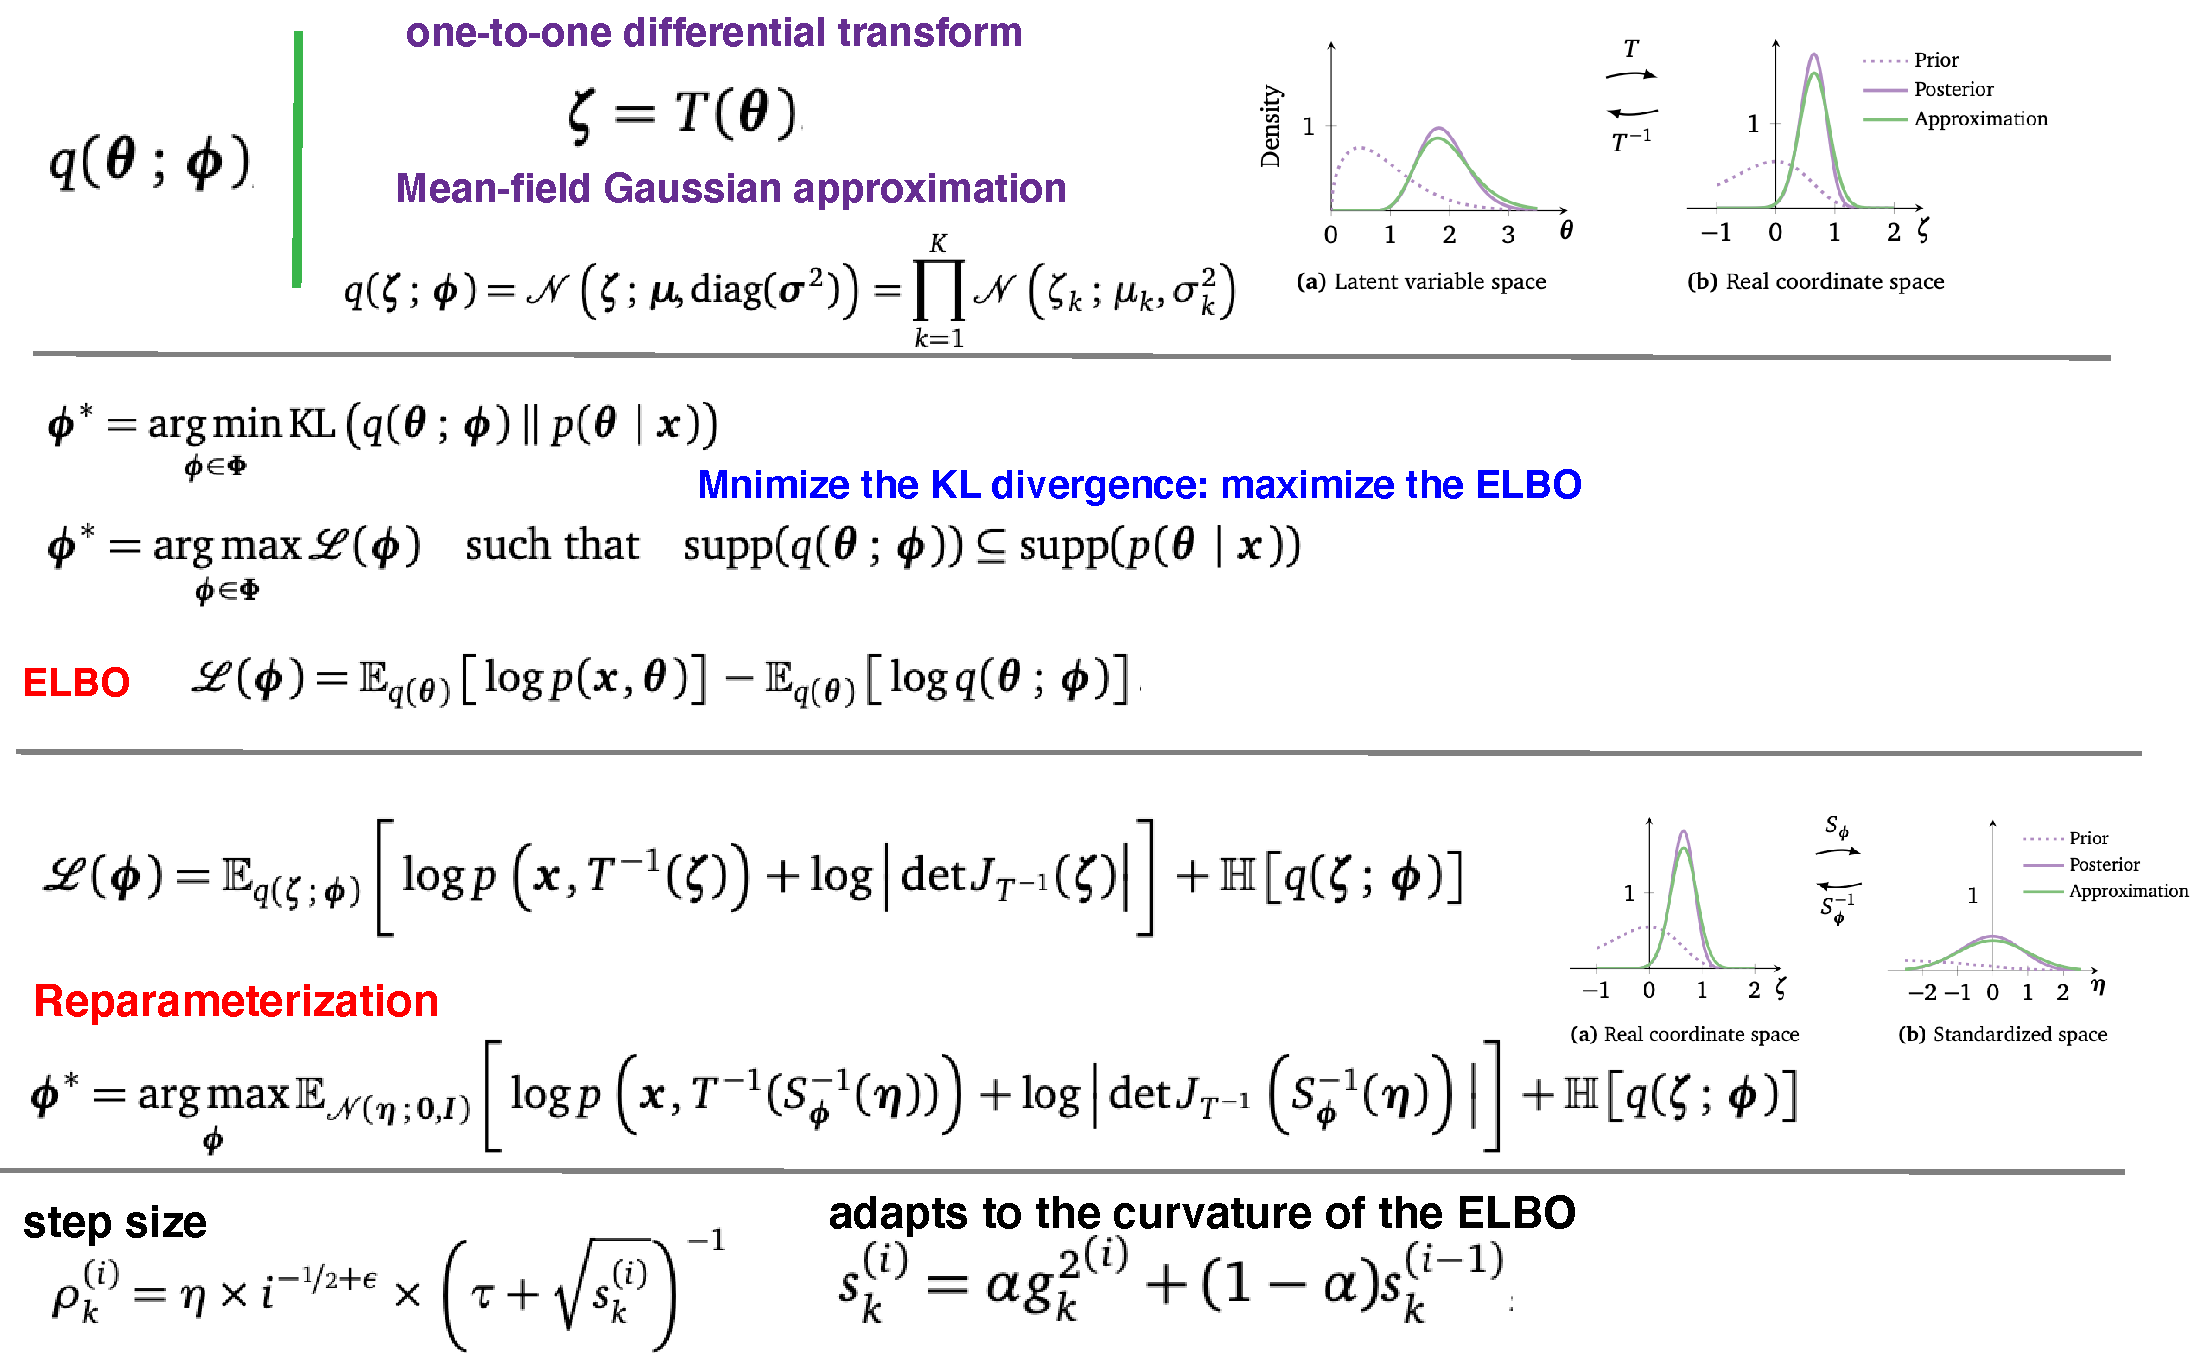
\includegraphics[width=0.9\textwidth]{advi}
  \end{figure}
\end{frame}

% \begin{frame}
  \frametitle{Pyro}
  Besides Stan, there are several probabilistic language programming libraries
  based on the deep neural network related framework, such as Pyro
  \cite{bingham2019pyro}, which is based on Pytorch.
  \begin{itemize}
  \item
    It fully supports GPU by Pytorch. So they can easily handle large scale of
    data sets.
  \item
    It supports variational inference (eg. VAE) and NUTS for sampling.
  \item
    It's easier to install and implement than Stan.
  \end{itemize}

  With the help of the scanpy \cite{wolf2018scanpy}, which is a Python package specific designed
  to handle large scale of scRNAseq dataset, we could write our method using Pyro
  when the model is mature.
\end{frame}


\section{References}
\begin{frame}[allowframebreaks]
  \bibliography{scRNASeq.bib}
\end{frame}

\end{document}